\chapter{Dawn, 1940-1960}
\section{Where Does it Start?}
There is significant debate about who created the first compiler,in no small
part due to ambiguous nomenclature.The term \textit{software} came into use
sometime between 1959 and 1962,as \citeauthor{the-first-computers-2002} note:
\begin{quotation}
  [Expressions] such as "hardware", "software", "machine language",
  "compiler", "architecture" and the like... were unknown in 1950.
  They only arrived a decade later, but the underlying concepts were
  quite familiar to us.
  \cite{the-first-computers-2002}
\end{quotation}

This Honeywell advertisement \textit{A Few Quick Facts on Software} sought to
clarify these terms as well:

\begin{quotation}
  Software is a new and important addition to the jargon of computer
  users and builders.It refers to the automatic programming aids that
  simplify the task of telling the computer 'hardware' how to do its
  job\dots
  % Generally there are three basic categories of software:
  % 1) Assembly Systems, 2) Compiler Systems, and 3) Operating Systems.
  \cite[ch.5]{new-history-of-modern-computing}
\end{quotation}

At this time, hardware was the only piece that mattered to customers.Software
was an afterthought, if a thought at all.The instruction set of the machine was
important, because that was the user's interface to the machine.It should come
as no surprise, then, that the origins of our modern understanding of the term
\textit{compiler} are similarly murky, especially considering the fact that
\textit{compiler} already carried meaning in English, and was repurposed for
computing. John Backus even pointed out how the ambiguity around the term
\textit{compiler}makes computing history ca 1950s especially difficult to
untangle:
\begin{quotation}
  There is an obstacle to understanding, now, developments in
  programming in the early 1950s. There was a rapid change in the
  meaning of some important terms during the 1950s. We tend to assume
  that the modern meaning of a word is the same one it had in an early
  paper, but this is sometimes not the case. Let me illustrate this
  point with examples concerning the word "compiler."
  \cite{Backus_1980_Programming_in_America_in_1950s}
\end{quotation}
\bigskip
Once could argue that any of these efforts constituted the first compiler:
\begin{itemize}
  \item Konrad Zuse's run-programs for the Z4 at the ETH Zurich in 1950
  \item Grace Hopper's A-0 and A-1 compilers for the UNIVAC I at
    Remington Rand in 1951
  \item Laning and Zierler's algebraic compiler for the Whirlwind at MIT in 1950
  \item John Backus's \FTNI{} compiler at IBM
\end{itemize}

I attempt to discuss these in order, however their efforts overlap
significantly in time.I try to tell their stories as a whole, though each story
contains references to the others;if you find yourself confused by names
introduced out of context, please finish the chapter or search for the content
within this chapter before giving up.
\section{Development of the Z4}
Konrad Zuse, a German civil engineer, began work on the Z4 during World War
II.Funded partially by his family and partially by the Nazi government, his
prior works demonstrated significant creativity and ingenuity, and they were
leveraged to build precursors to modern cruise missiles and guided bombs.Most of
Zuse's machines prior to the Z4 were destroyed during the war. \todo{Zuse's Z4
  was a strange machine with bespoke memory and instruction set.This
  affected how
the compilers for it were designed.} In a turn of events Konrad Zuse was made
aware of Aiken's Mark I through his daughter:
\begin{quotation}
  Konrad Zuse told me an amusing anecdote about how he first
  encountered the work of Aiken. The occasion of our conversation was
  a luncheon in Zuse's honor, hosted by Ralph Gomory at the Watson
  Research Laboratory of IBM before a lecture given by Zuse to the
  staff of the lab. When Zuse learned that I was gathering materials
  for a book on Aiken, he told me that he had come across Aiken and
  Mark I in an indirect manner, through the daughter of his
  bookkeeper. She was working for the German Secret
  Service (Geheimdienst) and knew through her father of Zuse's work on
  a large scale calculator. According to Zuse,the young woman never
  learned any details about his machine, which was shrouded in
  war-time secrecy. But she knew enough about Zuse's machine to
  recognize that the material filed in a certain drawer related to
  advice that seemed somewhat like Zuse's. She reported this event
  to her father, giving the file number of the drawer, and the father
  at once informed Zuse of her discovery. Zuse, of course, could not
  go to the Secret Service and ask for the document since that would
  give away the illegal source of his information. Zuse was well
  connected, however, and was able to send two of his assistants to
  the Secret Service, armed with an official demand for information
  from the Air Ministry,requesting any information that might be in
  the files concerning a device or machine in any way similar
  toZuse's.Zuse's assistants were at first informed that no such
  material existed in the files, but they persisted and eventually got
  to the right drawer. There they found a newspaper clipping (most
  likely from a Swiss newspaper), containing a picture of Mark I and a
  brief description about Aiken and the new machine. But there was not
  enough technical information to enable Zuse to learn the machine's
  architecture.
  \cite{howard_aiken_and_the_dawn_of_the_computer_age_2000}
\end{quotation}
\section{The ETH's Acquisition of the Z4}
There were several early efforts to create programs that produced punch
cards which contained machine code instructions, which could then be fed back
into the machine as input punchcards.The programs produced by these early
compilers were called \textit{run-programs}, and the process of using them was
called \textit{automatic programming}, a term later coined by Grace Hopper.The
first of these programs was run on a machine called the Z4, designed by Konrad
Zuse in Germany.Professor Eduard Stiefel, shortly after establishing the
Institute of Applied Mathematics to study numerical analysis at the Swiss
Federal Institute of Technology (ETH) in Zurich,began searching for a computer
for the institute.He learned of the computing advancements in the United
States, Great Britain, and Germany,but no machines were readily available at
the time. He sent his assistants Heinz Rutishauser and Ambros P. Speiser to the
US to study the latest developments in computing; they spent most of 1949
withHoward Aiken at Harvard and John von Neumann at Princeton.
\begin{quotation}
  Before we returned, that is, in the middle of 1949, Stiefel was informed
  about the existence of Konrad Zuse'sZ4. At that time Zuse was living in
  Hopferau, a German village near the Swiss border. Stiefel was told that the
  machine might be for sale. He visited Zuse, inspected the device, and reviewed
  the specifications.Despite the fact that the Z4 was only barely
  operational, he
  decided that the idea of transferring it to Zurich should by all means be
  considered. Stiefel wrote a letter to Rutishauser and me (we were at Harvard at the time), describing the situation and asking us to get Aiken's opinion.
  Aiken's reply was very critical - the future belonged to electronics
  and, rather
  than spending time on a relay calculator, we should now concentrate our efforts
  on building a computer of our own.
  \cite{konrad-zuses-z4-2000}
\end{quotation}
The Z4 was a bespoke machine with unique components; the computational logic
was wired together with telephone relays and the memory was entirely mechanical.
\begin{quotation}
  The Z4 could be used as a kind of manually triggered calculator: the
  operator could enter decimal numbers through the decimal keyboard, these
  were transformed into the floating point representation of the Z4, and were
  loaded to the CPU registers, first to OR-I, then to ORII. Then, it was possible
  to start an operation using the "operations keyboard" (an addition, for
  example). The result was held in OR-I and the user could continue loading
  numbers and computing. The result in OR-I could be made visible in decimal
  notation by transferring it to a decimal lamp array (at the push of a button).
  It could also be printed using an electric typewriter.
  \cite{architecture-of-konrad-zuses-z4-computer-2021}
\end{quotation}
It notably featured instructions for conditional branching and subroutine
calling, which both proved essential for the compiler development that would
follow at the ETH. Stiefel was undeterred by Aiken's criticism, and convinced
the ETH to purchase the Z4.In 1950, Heinz Rutishauser at Switzerland's ETH
obtains a Z4.
\begin{quotation}
  We also made some hardware changes. Rutishauser, who was exceptionally
  creative, devised a way of letting the Z4 run as a compiler, a mode
  of operation
  which Zuse had never intended. For this purpose, the necessary
  instructions were
  interpreted as numbers and stored in the memory. Then, a compiler
  program calculated the program and punched it out on a tape. All this required
  certain hardware changes. Rutishauser compiled a program with as many as 4000
  instructions. Zuse was quite impressed when we showed him this achievement.
  \cite{konrad-zuses-z4-2000}
\end{quotation}
Thus were the first run-programs produced.This is what we will
consider \textbf{the first compiler}, though it was not called that
at the time.Shortly after Stiefel's assistants' stints in the US and
correspondence with Aiken,one of Aiken's engineers would find
considerably more success exploring related ideas.
\section{Grace Hopper}
While Grace Hopper may not have been the first
to create a program that punched
out another program as its output, she pioneered the field of compilation to the
extent that many consider her the inventor of compilers.Her innovations were
also more readily adopted than those at the ETH.Consider Figure
\ref{fig:dawn-timeline}, and the pace of development in Hopper's time compared
to the years prior.Note that while we have ample data on \textit{how} Hopper's
compiler worked and how she and her team developed it, the intuition behind
those developments is foggy at best.We have recollections from Hopper and her
contemporaries, but only from long after the fact.It was not understood at the
time how important her work was, so we have only to speculate and piece together
oral histories.Originally a mathematics professor at Vassar College, Hopper
obtained waivers for her age and weight and joined the U.S. Navy in 1943,
eventually graduating first in her class from Midshipmen's School.She was
assigned, somewhat unexpectedly, to Commander Howard Aiken's Harvard
Computation Laboratory in 1944as the third programmer of the Automatic Sequence
Controlled Calculator (Mark I),the world's first operational computer.Although
it was significantly slower than the ENIAC, it was \textit{programmable};the
ENIAC had to be physically rewired to change its program.To write a compiler
for the ENIAC, one would need to plug the phone lines in the back of the
machine together to create the compiler, feed in the input program as data, and
a human operator would have to take the punchcards it produced and manually
rewire the machine to run that program.Aiken built the Mark I in collaboration
with IBM, though it is unclear how much either side contributed in its
development.The proportion of credit given to either party would be disputed in
numerous documents and press releases in the following years, including
the \textit{Manual of Operation for the Automatic Sequence Controlled
Calculator}, the technical manual for the Mark I.In the fall of 1944, Aiken
decided that his team needed to produce a book documenting the
technical developments at the Harvard Computation Laboratory and how the Mark I
was intended to be used.For this task, he chose Hopper; though she protested,
her reputation as a clear and thoughtful communicator and writer had already
earned her the job.Hopper was known for her writing ability, and it was a point
of emphasis in her teaching career.She would assign her mathematics students
onerous writing tasks to emphasize that"it was no use trying to learn math
unless they could communicate with other people."
\cite[interview on 5 July, 1972]{grace_hopper_and_the_invention_of_the_information_age_2009}

Aiken and Hopper both understood that, for the Mark I to be a success, it would be used
and understood by a large and diverse audience, and for that to happen, they
needed a detailed,compelling, and accessible
manual.\cite{annals_of_the_computation_laboratory_of_harvard_university_1946}:

% \todo{% ENIAC, could not be programmed (had to be rewired to be
% programmed)% but was real fast. Aiken's Mark I.% Fall 1944, Aiken
% wants to record technical developments at Harvard Computation
% Laboratory (as book),% chose Hopper, to her disagreement. Finished
% 561 page manuscript, published 1946.% She believed she was chosen
% for "clear, fluid prose."% her time as a math teacher made her good
% at writing/explaining things.% would force students to write essays
% on math topics and would grade harshely.% "it was no use trying to
% learn math unless they could communicate with other people."% Aiken
% and Hopper knew a large/diverse audience would need to understand
% it for it to% be successful; high value on good
% writing+communication.% Aiken's strict heirarchy+meritocracy
% allowed her to compete with the men.% IBM tried to steal all the
% credit for the Mark I from Aiken.% aiken distaste for being
% assigned woman officer, but meritocracy.% }

\section{Hopper and the Mark I's Manual}

Here we drift into some general computing history,
mostly because it was so formative for Hopper, who was in turn so
formative in the development of compilers.
Her manual for the Mark I
began with a detailed and dramatic retelling of computing history,
opening with the following quote from Charles Babbage
and culminating with the Mark I:

\begin{quotation}
  If, unwarned by my example, any man shall undertake
  and shall succeed in really constructing an engine embodying in
  itself the whole of the executive department of mathematical
  analysis upon different principles or by simpler mechanical means, I
  have no fear of leaving my reputation in his charge, for he alone
  will be fully able to appreciate the nature of my efforts and the
  value of their results.
\end{quotation}

Her history went on to cover:
\begin{itemize}
  \item Blaise Pascal's counting machines, "foundation on which
    nearly all mechanical
    calculating machines since have been constructed."
  \item Leibniz; stepped wheels system for mul/divs.
  \item Charles Babbage; most significant part of the manual dedicated to him.
    Difference engine, idea for computing machine. Invented punch card system to
    feed in information, made after textile looms. G H emphasized the
    machine would
    take 2 decks of cards, one for data, one for instructions (not
    von neumann).
  \item Ada King, Countess of Lovelace; series of essays on Babbage's machine.
    described possibly the first computer program. This could never
    run and would
    have to wait for the Mark I before the dream could come true.
  \item Aiken's Mark I
\end{itemize}

At one point, all new hires into Aiken's lab were
required to readCharles Babbage's autobiography.Hopper was first
exposed to Ada King in this text:"she wrote the first loop. I will
never forget; none of us ever will."Their coworkers in the Harvard
lab would jokingly cast Aiken as Babbage and Hopper as Ada King.Aiken
ran a rigidly hierarchical and meritocratic lab, which allowed
Hopper to produce quality work and placed her on more equal footing
with her male coworkers; Aiken openly disliked being assigned a female
officer,but Hopper's competence outweighed any such sentiments.Her
competence did not, however, shield her from the pressures of the
environment.She leveraged her computing knowledge to assist the war
effort,which included the bombing of Nagasaki.The stresses of the war
effort and Aiken's overbearing management drove her to substance abuse
in this time period.In 1946, Commander Edmund Berkeley wrote a report
on the conditions at theHarvard Computation Laboratory, which perhaps
contextualizes her incapacity to cope.

\begin{quotation}
  In his report, Berkeley systematically detailed the unfavorable
  conditions at the Computation Laboratory, including the length of
  the work day and the isolation of the staff from similar projects at
  MIT and the University ofPennsylvania. He named eleven talented
  people who had left or been dismissed byAiken between August 1945
  and May 1946, noting that all were "very bitter over the conditions
  on the project." The root of the problem, according to Berkeley,was
  that "in the Computation Laboratory there is no provision for
  appealing any decision or ruling whatsoever made by the project
  manager." He was amazed that no one at Harvard and no one in the
  Navy seemed to have jurisdiction over the rogue director, so that
  Aiken was able to rule with near absolute authority.
\end{quotation}

\section{Postwar Collaboration}

Hopper was relieved from active service in 1946, but she joined the Aiken's
lab to continue working on Aiken's Mark II (a paper-tape sequenced calculator)
andMark III (an electronic computer with magnetic drum storage).As the war
effort wound down, Aiken and his laboratory found themselves growing in
stature.He had the authority to move military personele to his Harvard
laboratory at his discretion, which he did.He also expanded the reach of his
lab's influence by opening up the computing community.During the war, research
and development of computers and programming was closely guarded, but after the
war ended, cross-organization collaboration was possible.Aiken started the
\textit{Symposium on Large Scale Digital Computing Machinery}in 1947 to foster
this collaboration.By this time there were numerous other organizations with
computing projects underway in the United States, which Aiken was now permitted
to collaborate with:

\begin{itemize}
  \item Eckert-Mauchly Computer Corporation (EMCC), BINAC and UNIVAC
  \item Harvard, Mark II and Mark III
  \item IBM, SSEC
  \item MIT, Whirlwind
  \item Institute for Advanced Study, MANIAC
  \item Engineering Research Associates (ERA)
\end{itemize}
\begin{quotation}
  We'd all been isolated during the war, you see, classified
  contracts and everything under the sun. It was time to get together
  and exchange information on the state of the art, so that we could
  all go on from there.
\end{quotation}

Hopper's postwar fellowship with the laboratory ended in 1949;after a
brief stint of unemployment, she joined a startup called the
Eckert-Mauchly Computer Corporation (EMCC)where she found a more
congenial environment to continue her work on compilers.

\begin{quotation}
  According to her friend and former Harvard colleague Edmund
  Berkeley, Hopper turned to alcohol during this period as a way to
  deal with the compounding pressures at the Harvard Computation
  Laboratory. She had dedicated herself fully to the overwhelming task
  of bringing Howard Aiken's machines to life.  She used the machines
  to solve critical military problems, including one that resulted in
  an explosion over Nagasaki. As the psychological strains
  became increasingly pronounced, alcohol seemed to serve as an
  effective outlet,freeing Hopper to express emotions and to
  temporarily forget obstacles real and imagined. According to
  Berkeley, the expiration of Hoppers Harvard research contract was
  the best thing that could have happened to her, although in
  the short term unemployment added to the stress.  During the last
  week of May 1949,the 43-year-old programmer packed up her
  belongings, headed to Philadelphia,and bet her future on two
  younger men who believed they could create the first commercial
  computer company.
  \cite{grace_hopper_and_the_invention_of_the_information_age_2009}
\end{quotation}

Once it was obvious to everyone in the industry that
Hopper was done at Harvard,she had a flurry of offers, but she chose
EMCC because of her impression of John Mauchly:

\begin{quotation}
In 1949 when people knew I had run out the time at
  Harvard, (and I guess everyone in the industry knew it) practically
  everyone asked me to come for interviews, including IBM. I went to
  the IBM headquarters and they gave me a huge [offer].  I was one of
  the very few people who did not work for IBM. I went for interviews
  with practically every computer manufacturer that there was at the
  time. Honeywell, RCA was thinking about it, Burroughs was in it.
  But it was John Mauchly I just couldn't miss. Working for him was
  obviously going to be a great pleasure. He was a wonderful guy, one
  of the best that ever lived.
  \cite{Hopper_1980_Oral_History}
\end{quotation}

\section{Hopper at the EMCC}

The company Hopper joined was one of the earliest pure computer-focused
ventures,founded by J. Presper Eckert Jr. and John Mauchly (designers of the
ENIAC, or the Electronic Numerical Integrator and Computer). This startup
environment contrasted sharply with the academic rigor of Harvard and the
industrial scale of IBM.There she found an open-minded and welcoming
environment to develop her ideas;Mauchly, who was to become Hopper's boss, was
characterized as"very broadminded, very gentle, very alive, very interested,
very forward looking,"
\cite{grace_hopper_and_the_invention_of_the_information_age_2009} creating a
tolerant, flexible company atmosphere in contrast to the pressure she
experienced at Harvard.A majority of their programming staff consisted of
mathematically inclined women who had served as ENIAC operators at the Moore
School.When Hopper arrived in 1949, EMCC had two major projects underway:the
BINAC (Binary Automatic Computer), which was close to completion,and the UNIVAC
I (Universal Automatic Computer), which would be running within a year.The work
environment and upcoming UNIVAC project excited Hopper and enticed her to join
the company after walking out of an interview with IBM; she felt that IBM was
too close to Aiken's lab. While the organization was grounds for fruitful and
innovative research and development team,EMCC was under financial strain; they
depended on partial payments for UNIVAC-I orders to stay afloat.The unexpected
death of EMCC's chairman Henry Straus forced Eckert and Mauchly to seek a
buyer,which they found in 1950 with Remington Rand, a typewriter and office
equipment manufacturer.In 1955, Remington Rand merged with Sperry Corporation
to form Sperry Rand.

\begin{quotation}
  Another Hopper programmer, Adele Mildred Koss, was assigned to Commonwealth
  Edison when the utility approached the Chicago sales office concerning a
  potential purchase of aUNIVAC for billing and payroll. At the time, Koss was 7
  months pregnant and working part time. Since her pregnancy precluded travel,
  Commonwealth Edison management was forced to come to Philadelphia in order to
  discuss their billing needs. In the end,the utility did not buy a UNIVAC, but
  instead purchased an IBM701 when it became available. Koss recalled: "I
  remember GraceHopper's memo to management saying 'This is a
  multi-million dollar
  client and you are not treating them like one. You have only assigned a part
  time programmer to work with.'"
  \cite[Adele Mildred Koss, interviewed by Kathy
  Kleiman]{grace_hopper_and_the_invention_of_the_information_age_2009}
\end{quotation}
Rand's team did not have nearly the programming expertise nor the personnel to
support their customers.Compounding with these challenges was the resistance
Hopper's team faced from the newRemington Rand management. Remington Rand was a
typewriter company and their management was far more familiar with the
mechanical punchcard technology of the previous generation of computers than
theUNIVAC's magnetic-tape memory.Even Thomas Watson Sr. had similar
inclinations about magnetic-tape memory:

\begin{quotation}
  Having built his career on punch cards, Dad distrusted magnetic
  tape instinctively. On a punch card, you had a piece of information that
  was permanent. You could see it and hold it in your hand. Even the enormous files
  the insurance companies kept could always be sampled and hand-checked
  by clerks. But with magnetic tape, your data were stored invisibly on a
  medium that was designed to be erased and
  reused.\cite{grace_hopper_and_the_invention_of_the_information_age_2009}
\end{quotation}
Hopper and her team at Remington Rand developed three "compilers"in rapid
succession, the A-0, A-1, and A-2, for the UNIVAC I.I quote "compilers" because
the A-0 and A-1 were not compilers in the modern sense.Her work was grounded in
intellectual openness, collaboration, and accessability;she pioneered the
debuggability of programming languages, compiler error reporting,and new ways
to share code and collaborate, for example.
\begin{quotation}
  Hopper's recollections point to motivations ranging from an altruistic
  desire to allow "plain, ordinary people"to program to dealing with her own
  laziness. Naturally one must be skeptical of such claims, for they were made
  years after the fact. In 1951 it was difficult for even a visionary like Hopper
  to imagine the eventual ubiquity of computer technology, and one can be pretty
  confident that Hopper was not a lazy person.
  \cite{grace_hopper_and_the_invention_of_the_information_age_2009}
\end{quotation}
Shortly after the fiasco with the utility company, Hopper's team was tasked
with supporting UNIVAC I customers at the US Census Bureau, a task she thought
no one in the company was prepared for. She began work on the A-0 in October
1951 in her spare time in order to address this mounting crisis facing
Remington Rand: they were unable to fully support their customers, and their
sales teams were, to put it kindly, incompetent with respect to their product,
and the sales team supported their customers as well as one might expect.
Management was as probably as receptive to her ideas about compilation as they
were to the UNIVAC I's magnetic-tape memory:

\begin{quotation}
  Inspired by Holberton's Sort-Merge Generator, Hopper conceived the
  idea of writing a
  program to create a program, or in modern day terms, building a compiler.
  The idea was to get commonly used subroutines automatically
  inserted into another program based on calculated offsets.
  Most people at the time considered this impossible.
  \cite{women_in_computing_history_2002}
\end{quotation}

As Hopper later recalled:
\begin{quotation}
  The Establishment promptly told us, at least they told me, quite
  frequently that a
  computer could not write a program; it was totally impossible; that
  all computers
  could do was arithmetic, and that it couldn't write programs.
  \cite{hopl_keynote}
\end{quotation}

Hopper was not the only member of the programming group with ideas about
programs generating other programs:

\begin{quotation}
  [Betty Holberton]'s retired. I think she's still part time at the
  National Bureau of Standards.
  Everybody's forgotten that she wrote the first program that wrote a
  program. She wrote that
  sort-merge generator, and what she did was feed in the specs for
  the data you were handling
  and the keys and that sort of thing, and then it generated the sort
  program for that specific data.
  That's the first time to my knowledge that anyone used the computer
  to write a program. Betty
  did that. I don't think she's ever fully received the credit for
  what she did in that case\dots

  I'm not sure that I would necessarily have gotten done what I did get done if
  she hadn't been ahead of me, so to speak. Knowing that she had used a program
  to generate a program, I had a good deal more nerve to go ahead and build the
  first A-O compiler.
\end{quotation}

Hopper and the team had decided that the atom of a programming language ought
to be the command imperative; verbs and nouns. All programmers, no matter
their native language, should be able to understand the verbs acting on nouns.
Thus they began working on their first mnemonics, the inputs to the A-0
compiler.

\section{The A-0 Compiler}

At this time we should note that the term \textit{compiler} had not yet taken
on its modern meaning. Hopper used the terms \textit{automatic programming} and
\textit{compiler} to refer to programs that produce other programs, but they
did not do the jobs that we associate with compilation today. Once Hopper and
her team had developed an environment of collaborative programming, they ran
into new problems with re-using each other's code.

\begin{quotation}
  On each of these routines they started with zero, which when you put them into
  a new program you had to add every one of the addresses to position it in the
  new program. Programmers could not add.  There sat that beautiful big machine
  whose sole job was to copy things and do addition. Why not make the
  computer do
  it? That's why I sat down and wrote the first compiler. It was very stupid.
  What I did was watch myself put together a program and make the computer do
  what I did.
  \cite{Hopper_1980_Oral_History}
\end{quotation}

John Backus had this to say about Hopper's A-2 compiler in 1976:
\begin{quotation}
  The above items give some idea of what the word "compiler" meant to one
  group in early 1954. It may amuse us today to find "compiler" used for such
  a system, but it is difficult for us to imagine the constraints and
  difficulties
  under which its authors worked
  \cite{Backus_1980_Programming_in_America_in_1950s}
\end{quotation}

Given that the A-2 was more sophisticated than the two prior iterations, this
should tell us something about how far their notion of a compiler was from our
present day understanding. Let us turn to the 1952 paper \textit{The Education
of a Computer} in which Hopper announced her A-0 compiler, which she presented
at a Pittsburgh ACM meeting\cite{education_of_a_computer_1952_hopper}.

\begin{figure}[h]
  \centering
  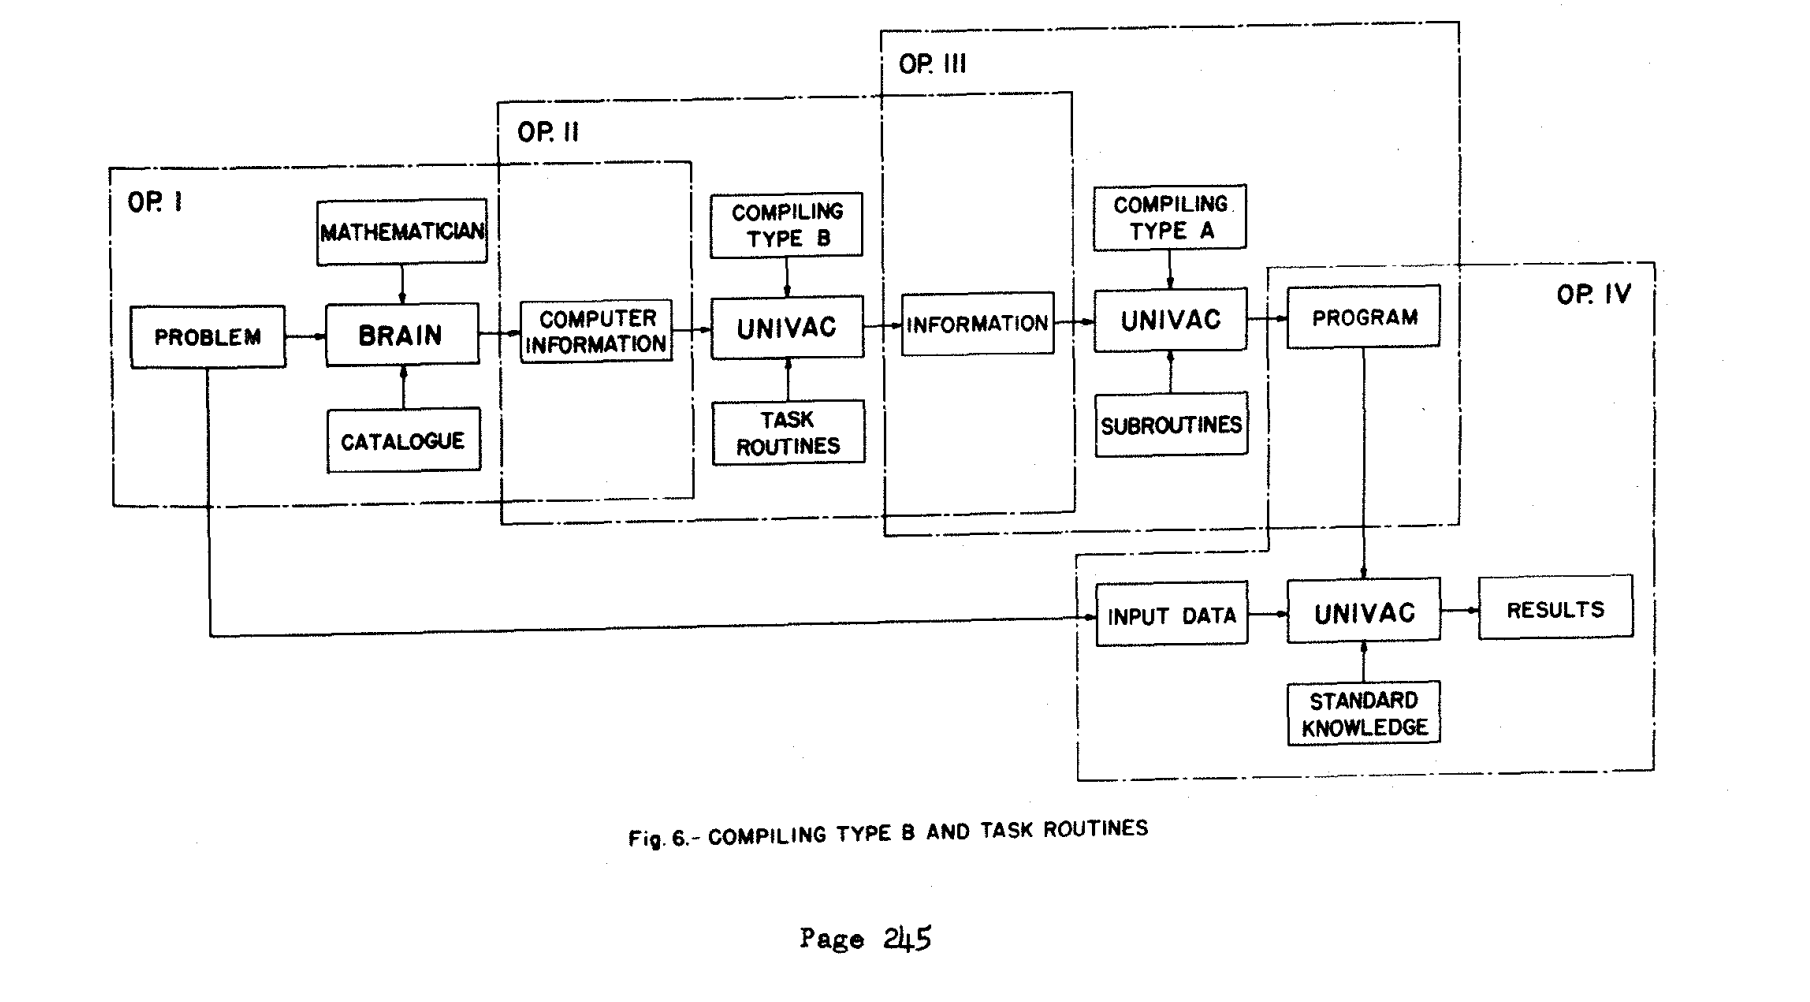
\includegraphics[width=.7\textwidth]{resource/gh_education_of_a_computer_type_fig_6.png}
  \caption{Depiction of \textit{type-B compilation} from Hopper's
  \textit{The Education of a Computer}}
  \label{fig:education-of-a-computer-1952-hopper-f6}
\end{figure}

In this paper, she dubbed her A-0 as a compiler because it was compiling subroutines from a
library into a program, adjusting offsets as necessary. This is far closer to
our modern notion of a linker; its role was to copy machine code from different
locations into a single output program based on an input program \textit{that
was still mostly in machine code}, save for the references to library
subroutines. Her notion of compilation was perhaps closer to the regular
English meaning of compilation, like that of compiling research papers into a
book. Her hope was that "the programmer may return to being a mathematician,"
though her A-0 did not lift the programmer away from machine code to nearly the
same extent as her subsequent efforts would
\cite{education_of_a_computer_1952_hopper}. 
One may also consider this effort
to be the first \textit{standard library}, which would become a major feature
of later compilers and programming languages. This set the stage for compilers
and programming languages providing a default set of useful routines for
programmers to pull from.

The cost of renting a computer remained high relative to the labor cost of
hiring a programmer, thus it was not always economical for computing centers to
use compilers at first. Richard Ridgway and several members of Hopper's team
began testing the A-0 against hand-written programs in the summer of 1952
\cite{ridgway_compiling_routines_1952}. For this study, Richard compared the
computer and labor time spent to calculate a table of values for the equation:

\[
y = e^{-x^2} \sin\left(\frac{x}{2}\right)
\quad \text{for } |x| < 1, \Delta x = 0.01.
\]

After an analysis of the same program written by hand and by the A-0, he
concluded that the A-0 (already considered "antique" by 1952, not more than two years
after Hopper began working on it) was cost-efficient to use for most workloads.
Richard writes in \textit{Compiling Routines}\cite{ridgway_compiling_routines_1952}:

\begin{quotation}
Thus, while more UNIVAC time may be required for the numerical solution of a 
problem as programmed by UNIVAC, more UNIVAC time, \underline{in toto}, is 
consumed by the conventional method. This remains true until the entire problem 
including tis self-contained repetitions is to be repeated, in this case at 
least eighteen times.

If the total preparation time is considered, the problem must be repeated some 
800 times before the conventional programming method overtakes the compiler 
method. In this case, the compiler used was the "antique," or A-0, the first to 
be constructed and the most inefficient.
\end{quotation}

\section{The A-1 and A-2 Compilers}

As Hopper and her team began work on the subsequent A-1 and A-2 compilers,
their motivations shifted away from reducing the tedium of programming to the
economic costs of programming (as is seen in Richard's report).
While computing time was initially far more
costly than human time, as the proportion of computing costs dedicated to human
labor increased over time, the importance of reducing human labor increased as
well.
Her team began working on the A-1 and A-2 in 1953, and the A-2 was
available to UNIVAC customers by the end of the year.
Hopper recruited Herbert Mitchell and Richard Woltman from Aiken's
lab to lead the development of the A-1 and A-2 compilers.
Margaret Harper, Frank Delaney, Mildred Koss, and Richard Ridgway were
the primary developers of these compilers.

There were a number of significant innovations between the A-0 and A-2.
The A-2 performed more of the jobs we associate with compilers today.
Most significantly, by 1954, the A-2 compiler accepted source code
in the form of \textit{pseudocode}, which was a (slightly) more human-friendly
format than plain machine code.
\todo{Some sources reference the A-2 compiler instruction manual,
but I'm unable to find this source online.}
John Backus described the A-2 compiler's 1954 May update as a significant
improvement because of these pseudocode instructions
\cite{hopl_backus_history_of_fortran}.
He placed the A-2 with Laning and Zierler's algebraic compiler and
his own \FTNI{} compiler as the primary compilers of significance in the
mid 1950s.

Along with pseudocode instructions, this compiler also produced
twelve-character error codes to inform the user why something went wrong
during compilation, which must have been tremendously helpful when users
had been accustomed to the alternative.
The compiler worked in two phases, first constructing an index of the
program and then producing the output machine code, informing the user as
it did so.
The a compiler should be friendly to its users was not necessarily a given at
the time; modern compiler tools owe this to Hopper (to the extend that they
are any better than the A-1).
Another feature of pseudocode instructions is that programs written 
in such a manner may be translated to run on different machines, provided
the compiler and standard library are available on those machines.
As far as we know, Hopper never attempted this, however.

By winter of 1953, the A-2 compiler was already being used heavily
by several institutions, including the US Census Bureau and
Lawrence Livermore National Laboratory.
Several of these provided feedback, bug reports, and occasionally features
back to the Remington Rand team.
Nora Moser of the Army Map Service sent Hopper a collection of comiler
improvements, library enhancements, and altogether new libraries in the
winter of 1954.
One cannot overlook the fact that Hopper was a woman in a male dominated
industry, and a number of other women in the industry were her early
collaborators.

Hopper presented on the A-2 at the Pentagon in 1953
\cite{pentagon_hopper_univac_workshop_1953},
facilitating communication with and amongst her users.
This was not the only time she sought to present her team's work
to a wider audience.
Non-UNIVAC customers also expressed interest; more government
agencies and potential customers (with existing IBM machines)
came to learn about their developments.
This open collaboration and sharing of information would set a precedent
for intellectual property in the budding software industry.
She had built the compilers as a way to make programming accessible
and facilitate the sharing of code, and this philosophy extended to
all sorts of information.
She had been successful in a more restricted environment at Harvard,
and she was able to see clearly the merits of a more open industry.

\section{After the A-2: A-3, AT-3, MATH-MATIC}

\todo{Should make some mention of interpreters in here.
Hopper made some observations that might be useful later.}

Not everyone was supportive of the advancements in compiler technology.
There was a significant chunk of the computing industry that thought
programming took too much creativity to be fully automated.
Hopper and John Backus found themselves on the same side of the debate,
both firm in their beliefs that computing should be made accessible.
This is a bit ironic, because IBM would shortly mount a significant effort
towards compilation and competition with Remington Rand, with Backus at the helm.

\begin{quotation}
    Just as freewheeling westerners developed a chauvinistic pride in their 
frontiersmanship and a corresponding conservatism, so many programmers of the 
freewheeling 1950s began to regard themselves as members of a priesthood 
guarding skills and mysteries far too complex for ordinary mortals.
\cite{Backus_1980_Programming_in_America_in_1950s}
\end{quotation}

Nonetheless, compiler development marched on and the number of compiler
developers continued to grow.
In 1954, Remington Rand formed the Automatic Programming Department
in support of Hopper's team.
With Hopper's ability to teach and communicate along with her compassion
for the programmer, the group thrived.
\todo{Adele Mildred Koss, interview by Kathy Kleiman, 1993,
talking about how nice it was to work for her.}
Just as Backus was inspired by Laning and Zierler's work at MIT, so too
was Hopper.
In preparation for the Office of Naval Research's 1954 Symposium,
her new department was focused on extending the A-3 compiler,
providing a compiler capable of generating more efficient machine code,
but not much else past what the A-2 could do.
Inspired by the work coming from MIT, they attempted to extend the A-3 to
support source code that resembled equations (more so than the three-address 
pseudocode that preceded it, at least).
This new compiler was called the AT-3 and formed one of the two major
components of the MATH-MATIC. The AT-3 was the \textit{Translator}
and the A-3 was the \textit{Arith-Matic Compiler}
\cite{ash_etal_1957_math-matic_manual}.

\begin{figure}[h]
    \centering
    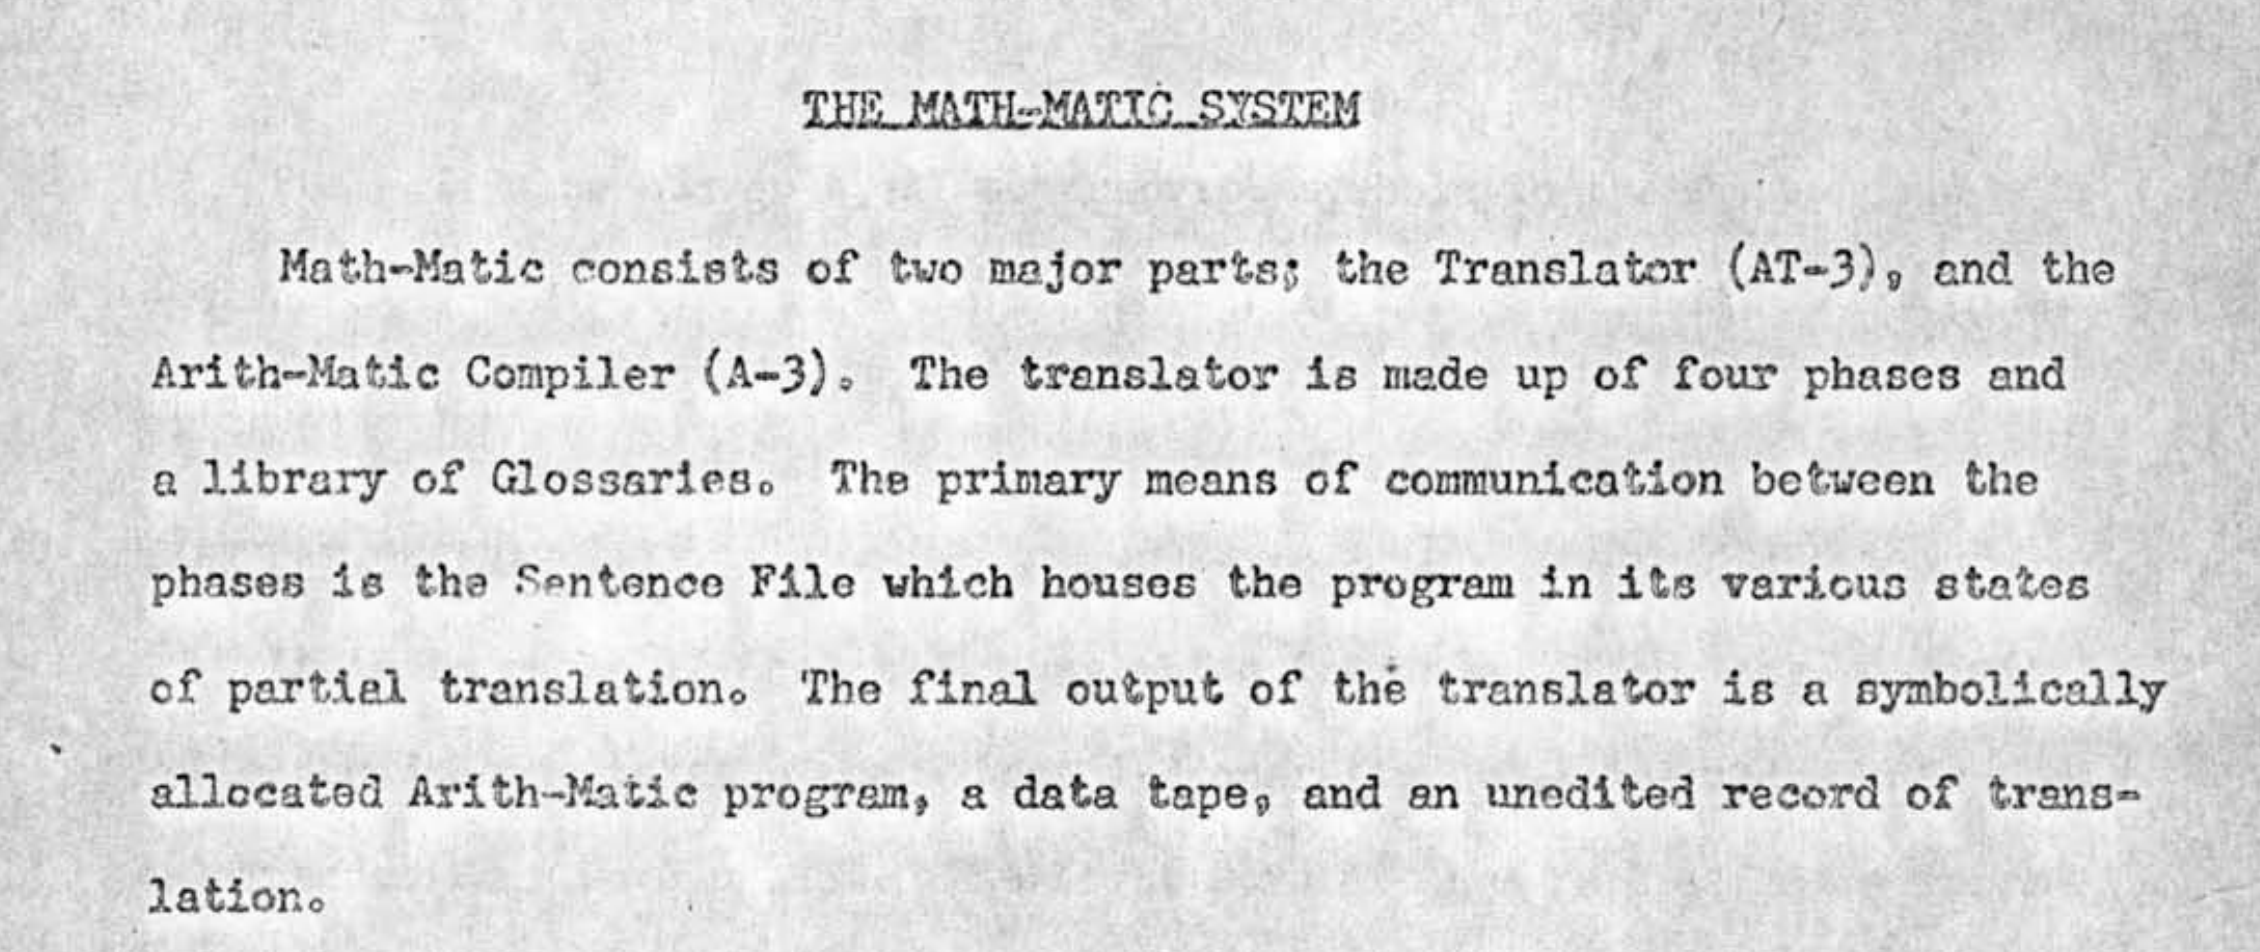
\includegraphics[width=.7\textwidth]{resource/mathmatic-user-guide.png}
    \caption{Excerpt from the MATH-MATIC User's Manual, 1957}
    \label{fig:mathmatic-user-manual}
\end{figure}

It is worth noting that \citetitle{grace_hopper_and_the_invention_of_the_information_age_2009}
\cite{grace_hopper_and_the_invention_of_the_information_age_2009}
appears to have a mistake regarding the A-3 and AT-3:

\begin{quotation}
Hopper and her colleagues explored the possibility of an
equation-based programming language, and by 1956 they had
modified A-3 to the point where it could support a user-friendly
source code. The resultant AT-3 compiler was later named
MATH-MATIC.
\end{quotation}

This led me to believe that the A-3 \textit{became} the AT-3 which was
renamed to the MATH-MATIC; however, the MATH-MATIC user manual
\cite{ash_etal_1957_math-matic_manual} specifies that the MATH-MATIC
is composed of the A-3 and the AT-3, which were apparently separate
programs with separate names (the Translator and the Arith-Matic Compiler,
respectively).
See Figure \ref{fig:mathmatic-user-manual}.
Knuth and Pardo describe the MATH-MATIC's development as:
"The language was originally called AT-3; but it received the catchier name 
MATH-MATIC in April, 1957, when its preliminary manual was released."
\cite{Knuth_TrabbPardo_1976_Early_Development}
Perhaps the \textit{language} A-3 was extended to become AT-3 which was
renamed MATH-MATIC, while the A-3 and AT-3 compiler programs remained
distinct; because I cannot find sources to clarify this nor the
original programs, I cannot conclusively describe the MATH-MATIC
and its precise relationship to the A-3 and AT-3 past what the
user's manual describes.

Because the MATH-MATIC translated source code into A-3 pseudocode
as an intermediate step, one might also consider this the first compiler
to have an internal intermediate representation.
The MATH-MATIC would last until about 1961, at which point UNIVAC users
were already expecting \FTN{} compilers available on their UNIVAC systems,
favoring IBM's language to Hopper's.

These layers of translation worked against them; the vast majority
of codes at the time were dominated by floating point arithmetic,
so any degradation of floating point performance would be catastrophic for the 
overall performance of the system.
Around the same time, John Backus had convinced IBM leadership that 
their new machine, the IBM 704, should have index registers and floating point 
processing hardware, which is exactly what both UNIVAC and IBM 701 customers
lacked and were spending all their time on.
Now that the 704 accounted for these prior deficiencies in both machines,
Backus's \FTN{} combined with the 704's hardware entirely outclassed the
UNIVAC I and Hopper's MATH-MATIC.

\begin{quotation}
But the MATH-MATIC programmers did not share the FORTRAN group's enthusiasm for 
efficient machine code; they translated MATH-MATIC source language into A-3 (an 
extension of A-2), and this produced extremely inefficient programs, especially 
considering the fact that arithmetic was all done by floating-point 
subroutines. The UNIVAC computer was no match for an IBM 704 even when it was 
expertly programmed, so MATH-MATIC was of limited utility.

Knuth and Pardo\cite{Knuth_TrabbPardo_1976_Early_Development}.
\end{quotation}

\section{The B-0, FLOW-MATIC, and COBOL}

In an interview for the Computer History Museum's Oral History series,
Hopper explains her motivations for the compilers to follow the A-2
\cite{Hopper_1980_Oral_History}:

\begin{quotation}
  \textbf{Pantages:} At that point did you have a feeling for what was 
happening, in terms of what you were contributing?

  \textbf{Hopper:} No. I've always objected to doing anything over again if I had 
already done it once. That was building the compiler. Then I decided there were 
two kinds of people in the world who were trying to use these things. One was 
people who liked using symbols - mathematicians and people like that. There was 
another bunch of people who were in data processing who hated symbols, and 
wanted words, word-oriented people very definitely. And that was the reason I 
thought we needed two languages.  The data processors did not like symbols, 
abbreviations that didn't convey anything to them.  They were totally 
accustomed to writing things in words. So why not give them a word-oriented 
language? And that was part of what was behind Flow-Matic B-0, which became one 
of the ancestors of COBOL.
\end{quotation}

\begin{figure}
    \centering
    \includegraphics[width=.7\textwidth]{resource/gh_data_processing_compiler.png}
    \caption{Depiction of Hopper's Data Processing Compiler\cite{hopper_1955_preliminary_definitions_data_processing_compiler}}
    \label{fig:data-processing-compiler}
\end{figure}

Hopper's interests in making programming accessible had not waned,
however her target audience shifted.
In January of 1955, she shared a her more radical ideas for a new
compiler in a report titled
\citetitle{hopper_1955_preliminary_definitions_data_processing_compiler}
\cite{hopper_1955_preliminary_definitions_data_processing_compiler}
.
This compiler would take on several names: first, the data-processing
compiler as outlined in the 1955 paper, then the B-0, the Procedure Translator,
and finally the FLOW-MATIC.

\begin{quotation}
  This was what she originally called the data processing compiler in January,
  1955; it was soon to be known as "B-0," later as the "Procedure
  Translator", and finally as FLOW-MATIC, This language used English
  words, somewhat as MATH-MATIC did but more so, and its operations concentrated
  on business applications.
  \cite{history_of_computing_in_the_twentieth_century_1980}
\end{quotation}

\begin{figure}[h]
    \centering
    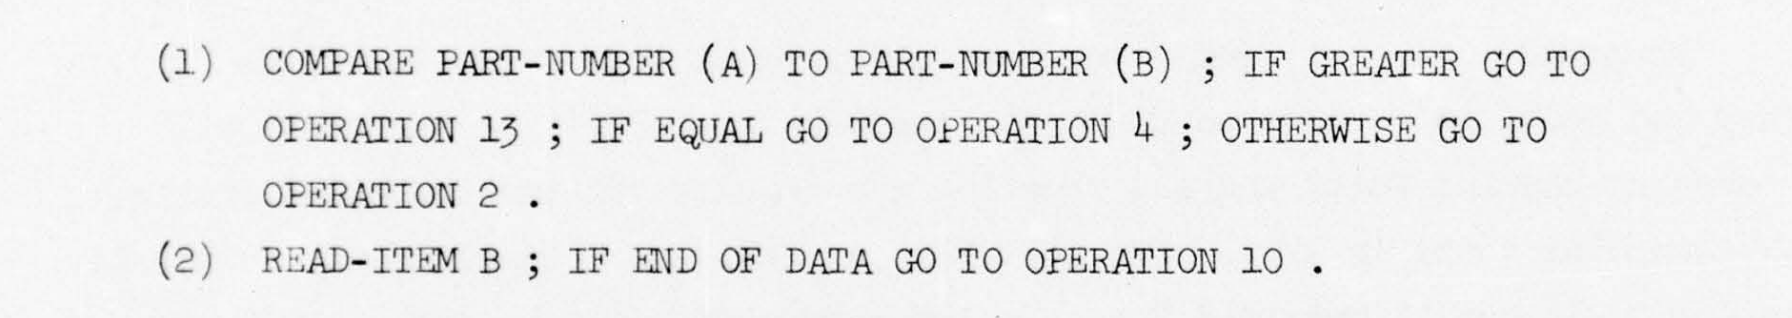
\includegraphics[width=.7\textwidth]{resource/flow-matic-example-knuth-pardo.png}
    \caption{Example FLOW-MATIC code from Knuth and Trabb Pardo\cite{Knuth_TrabbPardo_1976_Early_Development}}
    \label{fig:knuth-pardo-flow-matic-example}
\end{figure}

Always concerned with how intelligible her users would find her compilers
and programming languages, she focused more on business applications and managers.
Donald Knuth and Luis Trabb Pardo describe the FLOW-MATIC as
"far more influential and successful, since it broke important new ground."
\cite{Knuth_TrabbPardo_1976_Early_Development}
(see also Figure \ref{fig:knuth-pardo-flow-matic-example}).
Instead of catering her compilers to mathematicians and scientists
by introducing mathematical symbols and notation, she sent members of
her team to UNIVAC customers to learn about their \textit{business} needs.

\begin{figure}
    \centering
    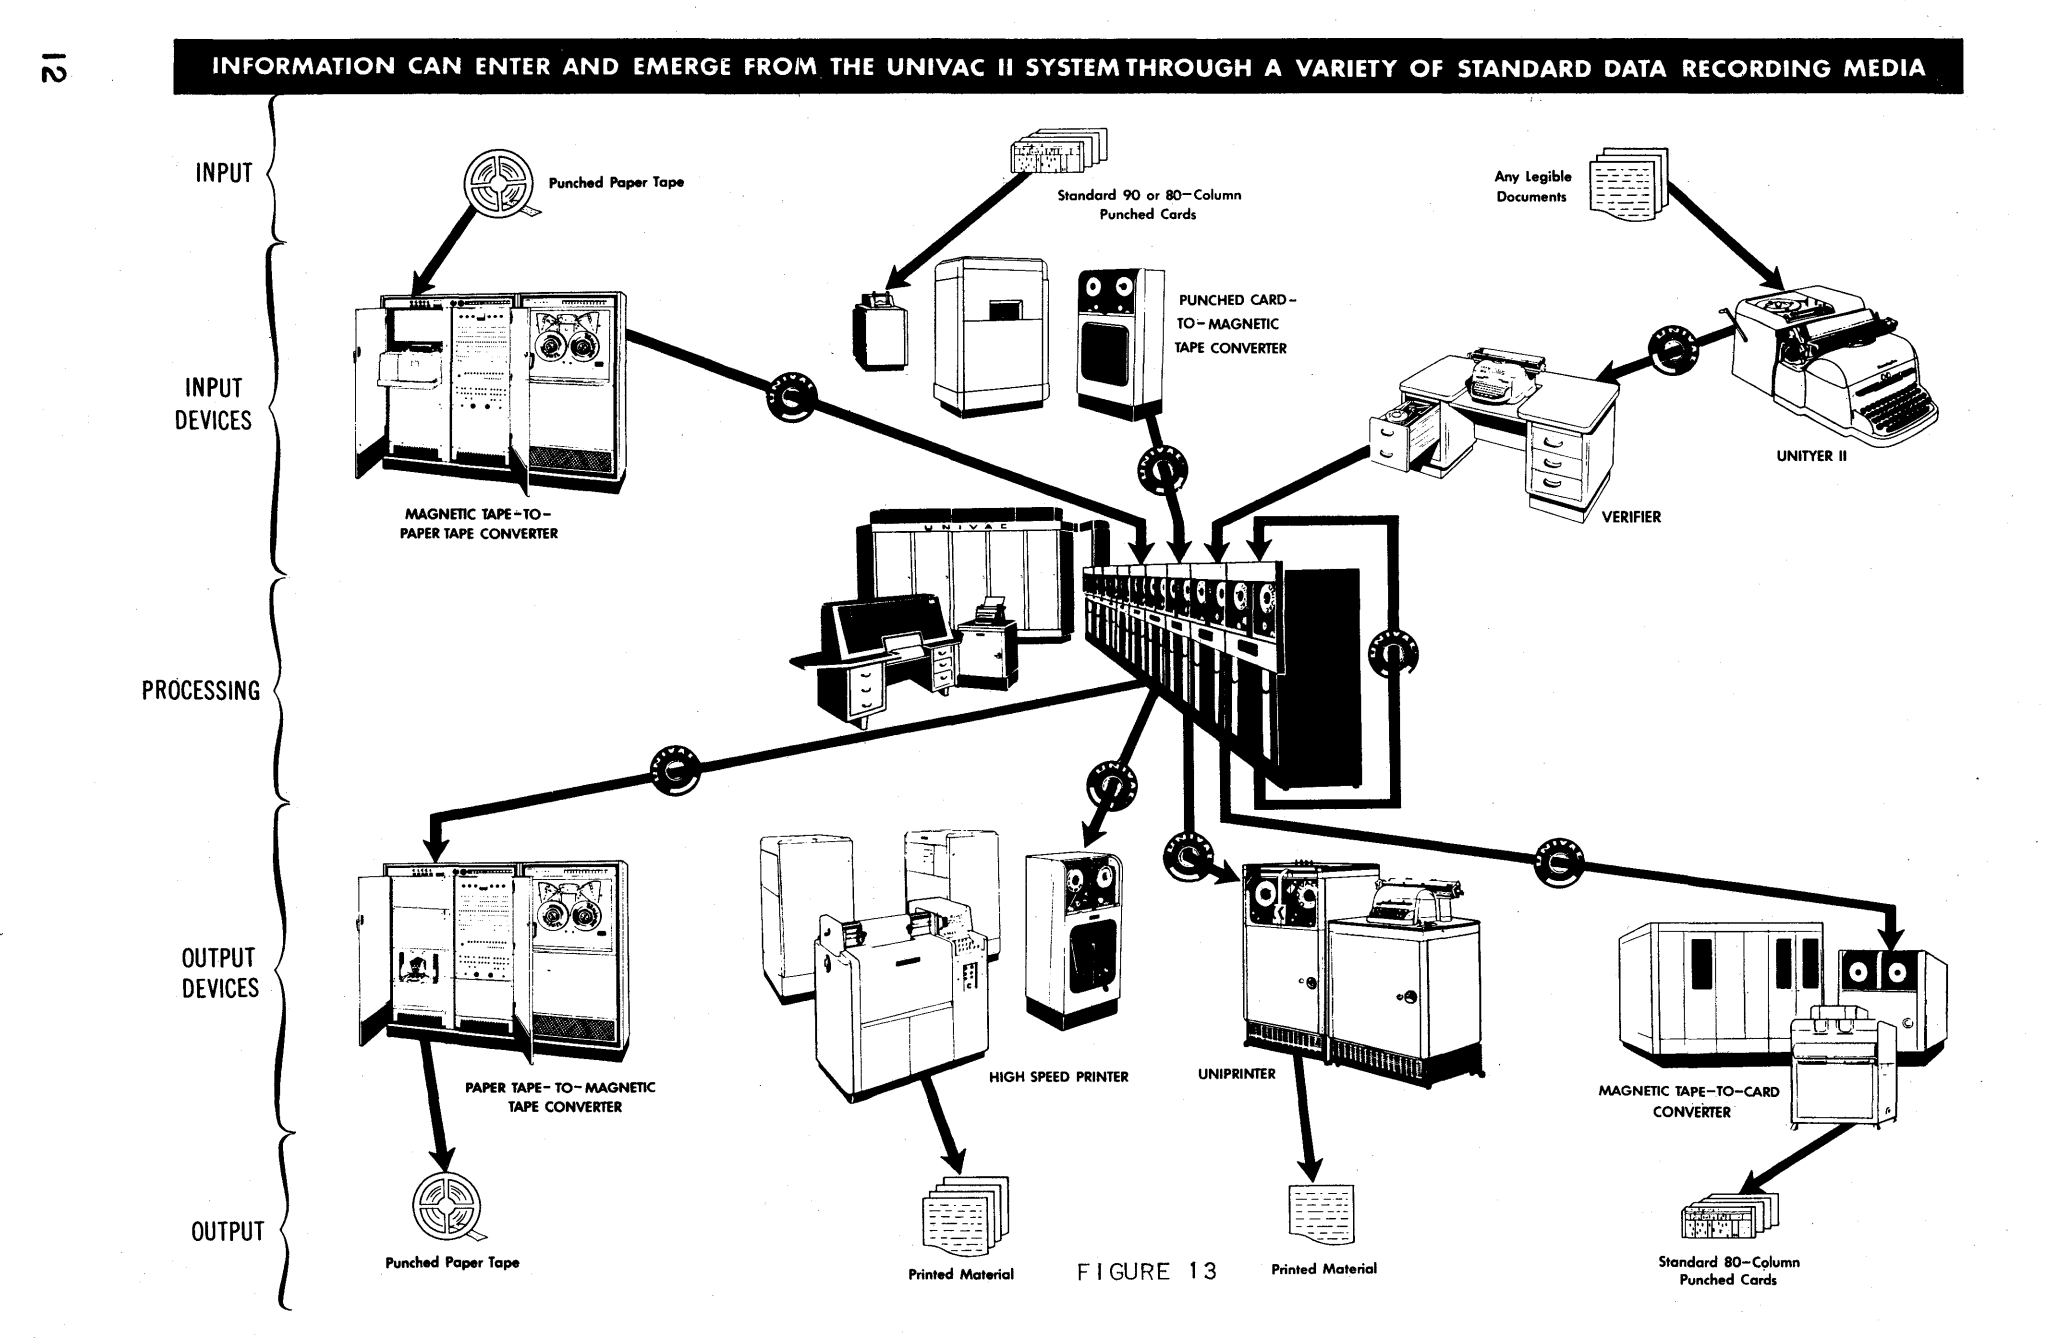
\includegraphics[width=.7\textwidth]{resource/flow-matic-ad-1959.png}
    \caption{Advertisement for FLOW-MATIC and UNIVAC II}
    \label{fig:flow-matic-ad-1959}
\end{figure}

The business compiler B-0 was first made available to UNIVAC customers
at the start of 1958.
Shortly thereafter, Remington Rand merged with Sperry Gyroscope to form Sperry Rand.
The marketing department of the newly formed company renamed the B-0
to FLOW-MATIC.
Catering to business users, the FLOW-MATIC was programmed in English-like
statements such as:
\texttt{IF EQUAL GO TO OPERATION 5 ; OTHERWISE GO TO OPERATION 2 .}
The group toyed with using abbreviations for common words, but
after studying their customer's programs, they found that too many
abbreviations could be mapped to different words based on the customer,
so the abbreviated form was abandoned.
Jean Sammet notes: "A preliminary manual
for the running system was marked Company Confidential and dated July,
1957; it was available to me at that time since I was an employee of the
Sperry Rand Corporation"
\cite{sammet_programming_languages_history_and_fundamentals_1969}.
The first generally available version of this document was available
in early 1958 in \citetitle{sperryrand_1959_flowmatic}\cite{sperryrand_1959_flowmatic}.
In this manual, one now finds advertisements for the UNIVAC II\ref{fig:flow-matic-ad-1959}.

In this document, one also finds a crude method for specifying the language,
which the reader should note; Backus would propose a more formal method
for specifying programming languages not long after this.
For example, the \texttt{CLOSE-OUT} command is specified in the FLOW-MATIC manual as
\footnote{The $\Delta$ symbols were present in the original manual because it signified
an empty space in the punchcards the FLOW-MATIC was written on}:

\[
\Delta \text{\texttt{CLOSE-OUT}} \Delta
\left[
\begin{array}{c}
  \text{file} \\
  \text{files}
\end{array}
\right]
\Delta
f_1
\Delta
\left[
f_2
\Delta
f_3
\Delta
\dots
\Delta
f_n
\right]
\]

There was no format method for specifying languages at the time.
In 1959, one of the B-0 developers, Mary Hawes, contacted Sperry Rand about a meeting to
discuss the direction of compilers for business applications.
\todo{In some places, Hawes is described as one of the B-0 developers which leads
me to believe she worked at RR or SR, but Sammet points out that she worked
for the ElectroData division of the Burroughs Corporation. Need to clarify.}
Sammet states\cite{sammet_early_history_of_cobol_1978} that Block's 1959 
\textit{Report on Meeting held at University of Pennsylvania Computing Center} names
Hawes as having called this meeting:

\begin{quotation}
\dots meeting was the result of a request by
Mary K. Hawes (ElectroData Division, Burroughs Corporation) to plan a formal meeting
involving both users and manufacturers where plans could be prepared to develop the
specifications for a common business language for automatic digital computers.
\end{quotation}

I am unable to retrieve this document; we will take Jean Sammet's word for it.
\todo{there is not much about Mary Hawes available online,
I can't even find the papers Hawes originally wrote.
Try to find \textit{Mary Hawes, “Automatic Routines for Commercial Installations”}}
Through a connection at the Department of Defense (Charles Phillips), this group
asked the DoD to sponsor the meetings and recommended a list of attendees, including
7 representatives from computer manufacturers and 14 from user organizations.
In an ACM talk on September 1, 1959, Phillips remarked that "embarrassed that 
the idea for such a common language had not had its origin by that time in 
Defense since we would benefit so greatly from the success of such a project."
\cite[Phillips, as quoted by Sammet in]{sammet_programming_languages_history_and_fundamentals_1969}.
There was a great deal of discussion around a common business language
that could be shared across different computer systems and reduce the overall cost of programming.
\textit{Three separate committees} were formed for this purpose; a short, medium, and long-term committee.
Sammet remarks that "the importance of the notion of Short and 
Intermediate-Range Committees is absolutely crucial to an understanding of the 
development of COBOL"\cite{sammet_early_history_of_cobol_1978}.
She went on to say:

\begin{quotation}
This wording is clearly ambiguous, and at the time, there was some discussion 
as to whether or not we were to try and create a language. It was by no means 
clear \textit{then} that we were to do anything \textit{except} try and 
\textit{combine} the three known languages of the time.
These were FLOW-MATIC, \dots AIMACO, \dots and COMTRAN
\end{quotation}

AIMACO was a language developed at the Air Force, and COMTRAN (renamed to Commercial Translator)
existed only in an IBM manual whose implementation had never even started.
Clearly, Hopper and Sperry Rand's FLOW-MATIC was the most mature of these languages.
Indeed, Hopper pointed out that the language resulting from these committees
was almost entirely FLOW-MATIC\cite{Hopper_1980_Oral_History}, though the committee notes
did not say as much. Hopper's lack of an ego and her diplomatic skills
led her to give credit liberally in order to drive consensus.

\begin{quotation}
We'd written FLOW-MATIC before that, and if you take the FLOW-MATIC
manual and compare it with COBOL 60 you'll find COBOL 60 is 95\% FLOW-MATIC. So the
influence of Commercial Translator in fact was extremely small. But I figured the thing to do was
corral those people and when we had something to say, we'd say it was a compound of FLOW-MATIC
and Commercial Translator and keep the other people happy and wouldn't try to knock
us out. We'd give them some credit and they'd have to get on board with us. But if you compare
the two manuals you'd find that it had hardly any influence at all. But if you gave them credit for
it, why they'd go right along with you. If you didn't, they'd fight you. You can always give credit,
you can always afford to.

That again is the practical. Think about the other guy and his position and his interest. You are
always trying to work with people rather than against them. You've got a new idea; give the
boss credit for it. It doesn't cost you anything. 
\end{quotation}

Here the reader should note Sammet's observation of the differing goals of the three committees:

\begin{quotation}
I am certainly convinced in my own mind that had the Short-Range Committee 
realized at the outset that the language it created (i.e., COBOL) was going to 
be in use for such a long period of time, it would have gone about the task 
quite differently and produced a rather different result. But I believe that 
most of us viewed our work as a stopgap measure--a very important stopgap 
indeed, but not something intended for longevity.
\end{quotation}

Most of the disdain for COBOL may indeed come from the fact that it was designed by the \textit{short term}
committee, which was solely trying to combine the existing compiler and programming language practices
of the time into one language to prevent further bifurcation.
If COBOL seems like a mishmash of different ideas designed by committee without proper
foresight or thoughtful design, well, it more or less was.
Yet another committee was formed on top of these three, the "Committee on Data Systems Languages"
or CODASYL, which would be the exeucutive committee steering the direction of the other three.

\section{COBOL Comes Into Focus}

Throughout September and October of 1959, the short-term committee met
regularly to build consensus around this new language.
There were a number of similar names considered before settling on COBOL:

\[
\begin{array}{ll}
\text{BUSY}   & \text{Business System} \\
\text{BUSYL}  & \text{Business System Language} \\
\text{INFOSYL} & \text{Information System Language} \\
\text{DATASYL} & \text{Data System Language} \\
\text{COSYL}  & \text{Common Systems Language} \\
\text{COCOSYL} & \text{Common Computer Systems Language} \\
\end{array}
\]

On September 18th of that year, the committee settled on
COBOL, according to Jean Sammet's personal notes\cite{sammet_early_history_of_cobol_1978}.
I spare the reader of the full details of the committee's meetings,
and encourage interested readers to consult Sammet's detailed notes on the proceedings.
Perhaps the most important conclusion from these meetings was that there existed a
\textit{Basic COBOL}, and that no computer manufacturer could claim to support COBOL
unless they supported this core subset of the language.
This set the stage for numerous modern programming languages that contain a
standard language specification that all compilers must support to claim to
be a compiler for that language, key examples being C and C++.

The first correct and complete compilation of a COBOL program was performed in
August of 1960 on an RCA 501.
In December of that year Sperry Rand and RCA each wrote COBOL programs,
ran them on their own machines, exchanged programs, and verified that they ran on
the other manufacturer's machine as well (a UNIVAC II and an RCA 501).
Thus was the first programming language standardized to the point that different compilers
running on different machines could compile the same program correctly.

While Hopper's legacy tends to be tied to COBOL, I believe her true legacy lies in
her passion for open collaboration and making programming accessible.
She thought deeply about the needs of her users; she sent employees to study them
and learn what their pain points were and how best the compiler developers could serve them.
She considered how to tailor her technology to her users, how to make her compilers
more friendly speakers of other languages, and how to make compilers produce understandable
error message and make them more debuggable.
She facilitated communication between users and developers and advocated for
a liberal notion of intellectual property to facilitate the sharing of ideas and programs;
this outlook would lead to a cambrian explosion of compiler technology in the open-source era
decades after her work on COBOL.
This is where I think Grace Hopper's true legacy lies, not solely in the language
cobbled together by a potpourri of committees with a short-term view.

\section{Laning and Zierler at MIT}
\label{sec:laning-zierler}

\todo{Backus was a huge fan of thier work. Look at \citetitle{hopl_backus_history_of_fortran}.}
\todo{ Laning and Zierler, 1954. Early 1950s. Inspiration for Backus/\FTN{}.
Worked more like a modern compiler than Hopper's A-0 and A-1.  }

Backus on the Whirlwind\cite{Backus_1980_Programming_in_America_in_1950s}:
\begin{quotation}
  \textbf{5. The Priesthood versus the Laning and Zierler Algebraic Compiler}
  Very early in the 1950s, J. Halcombe Laning, Jr., recognized that
  programming using algebraic expressions would be an important improvement.
  As a result of that insight he and Neal Zierler had the first
  algebraic compiler
  running on WHIRLWIND at MIT in January 1954 [3]. (A private
    communication from the Charles Stark Draper Laboratory indicates
    that they had
  demonstrated algebraic compiling sometime in 1952!) The priesthood
  ignored Laning's insight for a long time. A 1954 article by Charles W. Adams
  and Laning (presented by Adams at the ONR symposium) devotes less than
  3 out of 28 pages to Laning's algebraic system; the rest are devoted to other
  MIT systems. The complete description of the system's method of operation
  as given there is the following
\end{quotation}

\begin{quotation}
  In retrospect, the biggest event of the 1954 symposium on automatic
  programming
  was the announcement of a system that J. Halcombe Laning, Jr. and Niel Zierler
  had recently implemented for the Whirlwind computer at M.I.T.  However, the
  significance of that announcement is not especially evident from the published
  proceedings [NA 524-], 97\% of which are devoted to enthusiastic description s
  of assemblers, interpreters, and 1954-style "compilers".
  \cite{Knuth_TrabbPardo_1976_Early_Development}
\end{quotation}

\begin{figure}[h!]
  \centering
  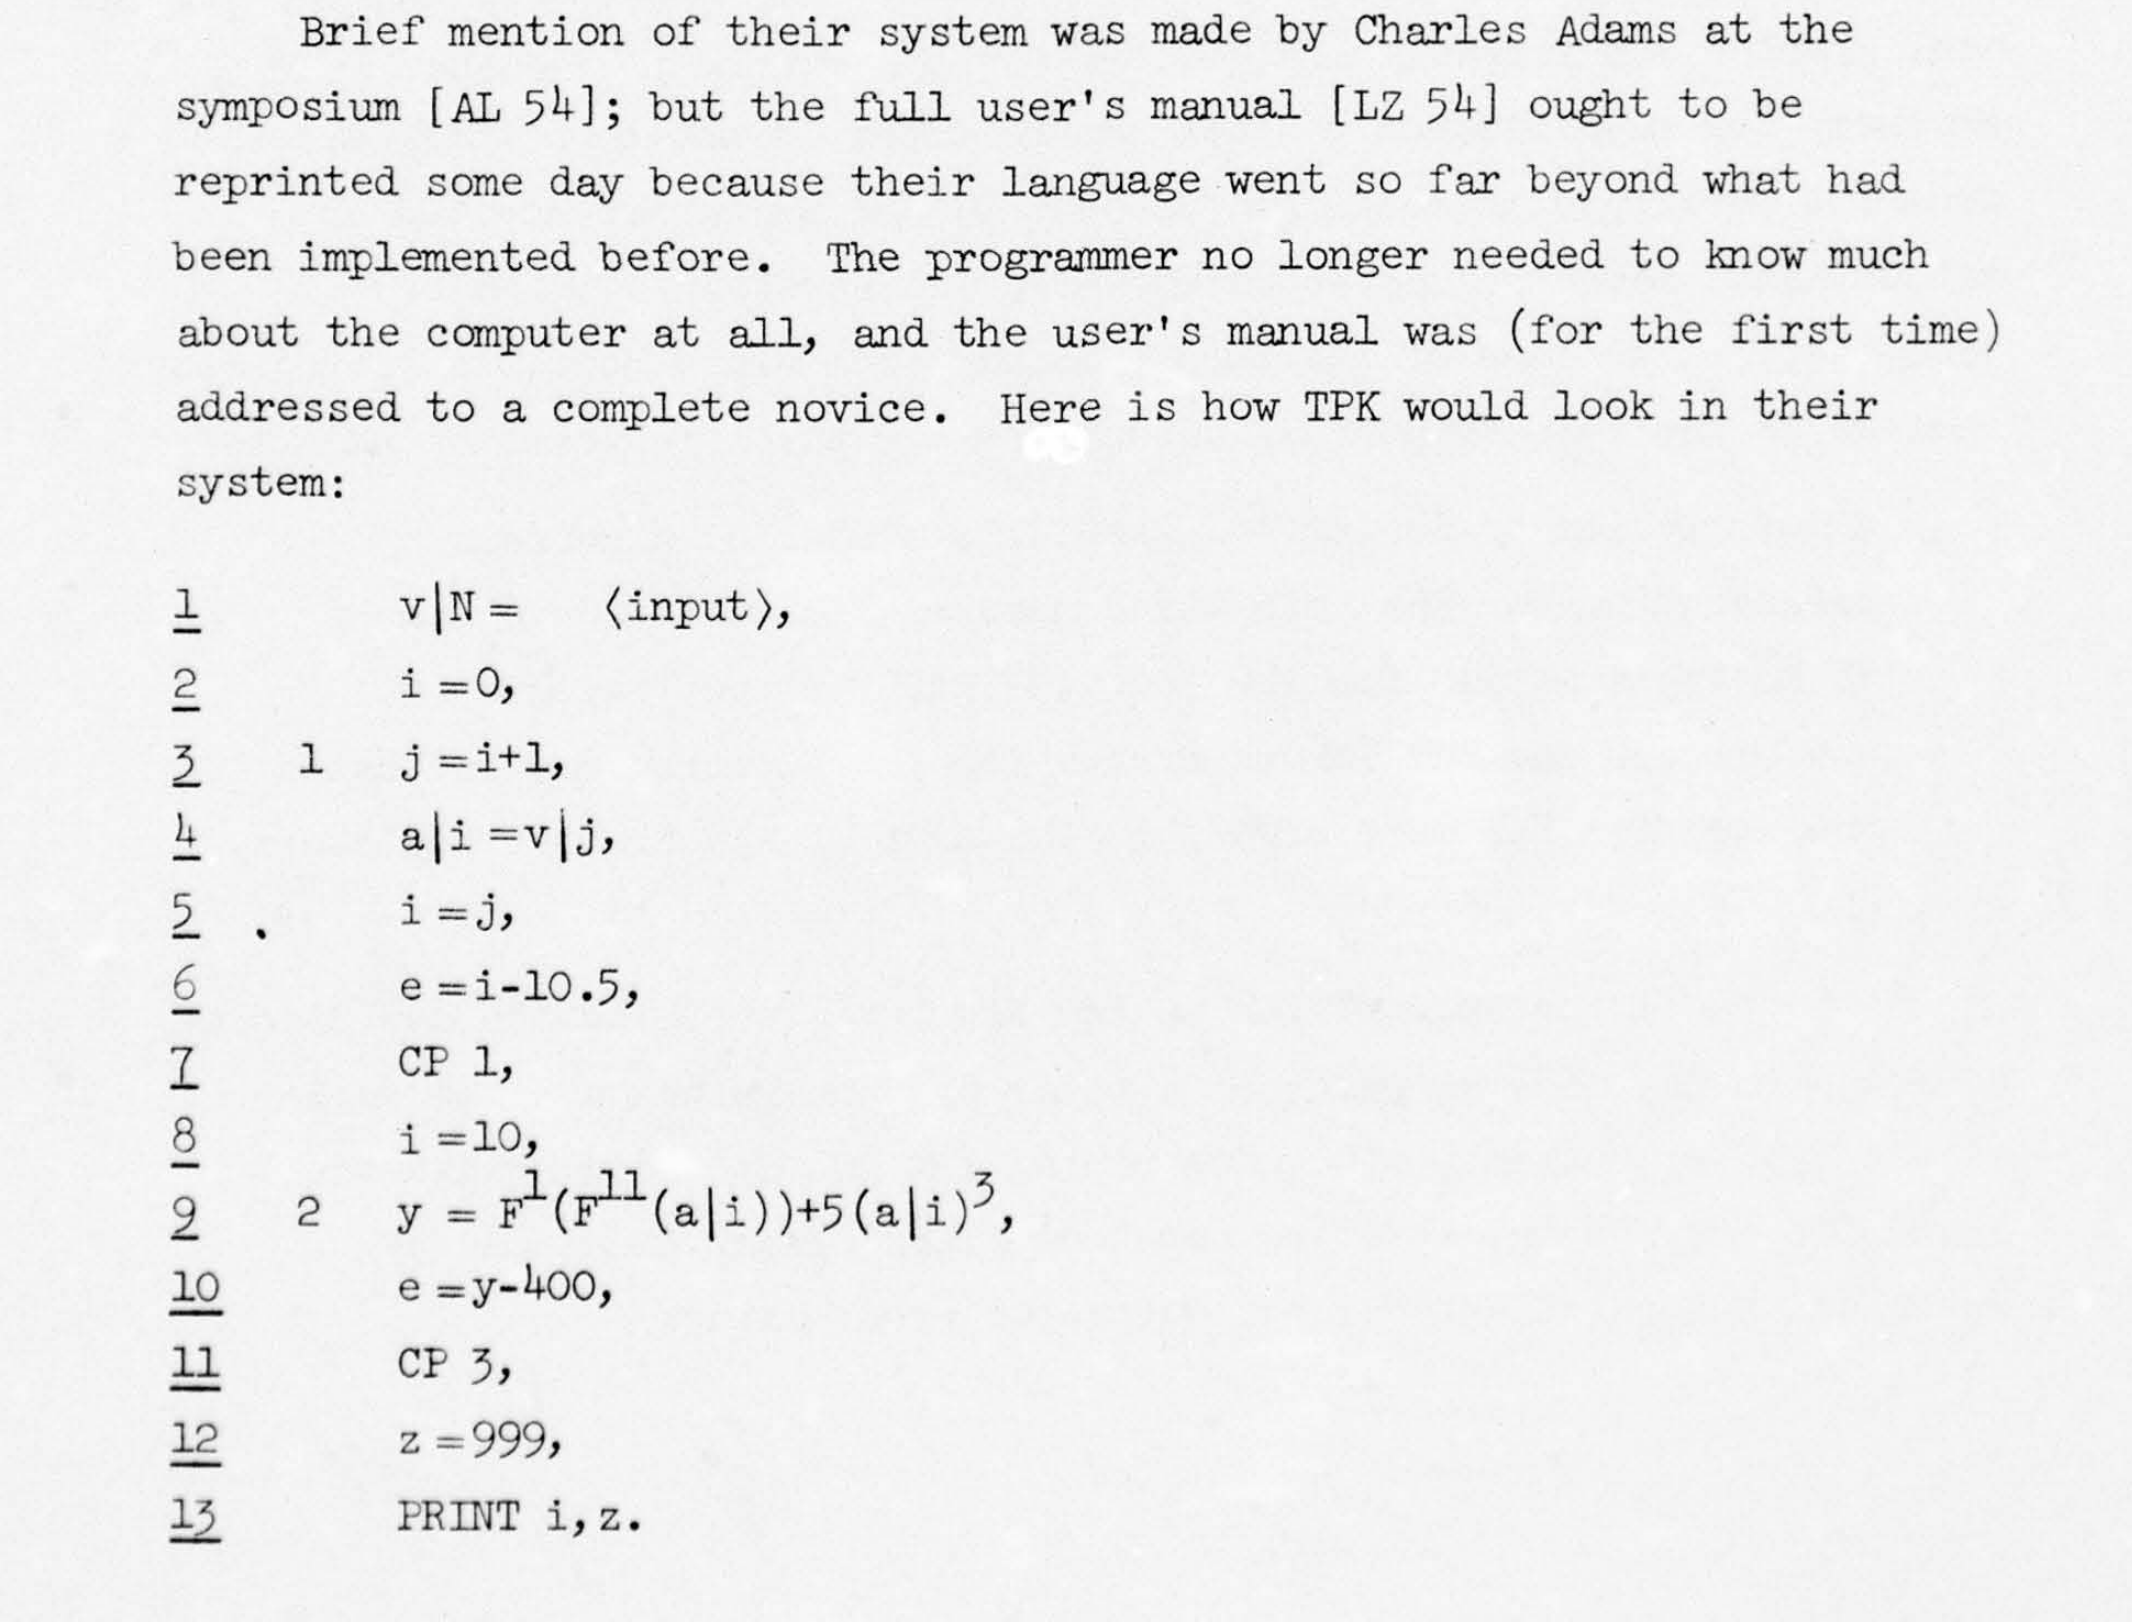
\includegraphics[width=0.5\linewidth]{resource/knuth_pardo_on_laning_zierlers_algebraic_compiler.png}
  \caption{Knuth and Trabb Pardo on Laning and Zierler's Algebraic Compiler}
  \label{fig:knuth-pardo-on-laning-zierler}
\end{figure}

\begin{quotation}
  The first programming system to operate in the sense of a modern compiler was
  developed by J. H. Laning and N. Zierler for the Whirlwind computer at the
  Massachusetts Institute of Technology in the early 1950s. They described their
  system, which never had a name, in an elegant and terse manual entitled "A
  Program for Translation of Mathematical Equations for Whirlwind I,"
  distributed
  by MIT to about one-hundred locations in January 1954.26 It was, in John
  Backus's words, "an elegant concept elegantly realized." Unlike the UNIVAC
  compilers, this system worked much as modern compilers work; that is, it took
  as its input commands entered by a user, and generated as output fresh and
  novel machine code, which not only executed those commands but also kept track
  of storage locations, handled repetitive loops, and did other housekeeping
  chores. Laning and Zierler's "Algebraic System" took commands typed
  in familiar
  algebraic form and translated them into machine codes that Whirlwind could
  execute.27 (There was still some ambiguity as to the terminology: while Laning
    and Zierler used the word "translate" in the title of their manual, in the
  Abstract they call it an "interpretive program.")28
  \cite{new-history-of-modern-computing}
\end{quotation}

\section{John Backus}

IBM did not feel that Aiken and the Harvard Computation Laboratory had given
them sufficient credit for their contributions to the Mark I, which left
Thomas Watson Sr. and the IBM folks bitter about the experience and eager to
produce a new device entirely in-house. This device would become the Selective
Sequence Electronic Calculator, or the SSEC. It was built on 57th Street in
Manhattan, and it was monstrous. Roughly 50 by 100 feet with a giant console
and hundreds of toggle switches and tape units and relays behind glass panels;
there were giant windows that allowed passersby to see the machine in action.

One such passerby was John Backus, a recent Masters graduate from Columbia
University. He was intrigued by the machine, which he mentioned to his tour
guide, who suggested he go upstairs and talk to the boss about it. Robert "Rex"
Seeber gave him a puzzle, which he solved, and he was hired on the spot
\cite{backus_oral_history_2006}.

In 1942, Backus majored in Chemistry at the University of Virginia where he
struggled academically. He was expelled due to poor attendance within the first
year before being drafted into the US Army. He commanded an antiaircraft
battery at Fort Steward, Georgia, remaining in the US for the remainder of
WWII.

While he did not at first find success in academia, he got very good marks on
military aptitude tests. He was directed to the University of Pittsburgh's
engineering program and later to a premedical program at Haverford College near
Philadelphia (which is where he grew up). In 1945 he attended the Flower and
Fifth Avenue Medical School in NYC, but he was still struggling with the
academy. He was uninterested in medicine, feeling that it was all about
memorization. He dropped out after less than a year.

He entered a radio technician school and became interested in math, which led
him to enroll in the math program at Columbia University. The SSEC that would
intrigue him at the IBM computing center was designed at the Watson Scientific
Computing Laboratory at Columbia.

\section{IBM Mathematical FORmula TRANslating System}

At IBM, Backus worked on the SSEC and later the IBM 701 and 704. The main use
of the SSEC was aerospace calculations; programming calculations to predict the
position of the moon was one of the first tasks he was given at IBM. He would
continue writing programs for these machines in spite of their poor usability.
His team's techniques would be used in the lunar missions of the 1960s.

The pain of writing programs for these early machines entirely in machine code
drove him to explore new ways to program. The first of these was a symbolic
notation for floating point arithmetic and address expression calculation
called Speedcoding\cite{backus_oral_history_2006}:

\begin{quotation}
  \textbf{Grady Booch:}
  So then from your experience with the SSEC, you then went on to
  produce Speedcoding, the
  Speedcoder\dots
  What were sort of the things that influenced you to create that in
  the first place?

  \textbf{John Backus:}
  Well, programming in machine code was a pretty lousy business to
  engage in, trying to figure
  out how to do stuff. I mean, all that was available was a sort of a
  very crude assembly program. So I
  figured, well, let's make it a little easier. I mean it was a
  rotten design, if I may say so, but it was better
  than coding in machine language.
\end{quotation}

The IBM 701 did not have an index register, so calculating addresses for array
operations was tedious and error-prone. Speedcoding provided a way to express
these calculations symbolically.

\begin{figure}[h!]
  \centering
  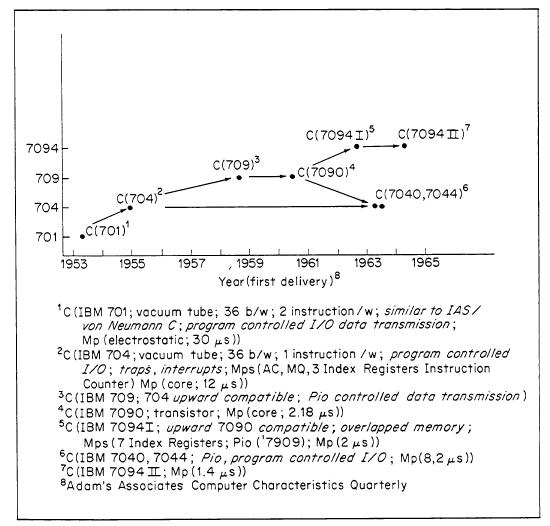
\includegraphics[width=0.5\linewidth]{resource/ibm-7094.jpeg}
  \caption{Excerpt from \textit{The IBM 701--7094 II Sequence: A
    Family by Evolution}
    \cite{Hamming_Feigenbaum_1971_IBM7094}, illustrating the
  instruction structure for summing quantities.}
  \label{fig:ibm7094-example}
\end{figure}

The 704 was the first machine to have such a register; it also had floating
point instructions and core memory, more or less obviating the need for
Speedcoding: "we were moving to the 704, which had built in floating point,
built in index registers, which was all that Speedcoding was supposed to
supply. So what the hell?" \cite{backus_oral_history_2006} He credits himself
with getting index registers and floating point into the 704.

%Here is an example from the IBM Speedcode manual\cite{IBM_1954_Speedcoding}:
%\begin{quotation}
%    Assume that it is necessary to compute the sum of 34 quantities stored in
%    locations 688 through 721 and to store the sum in cell 945.
% Assume further that
%    cell 1013 contains the number zero and that instruction 416 is the next
%    instruction to be executed. The sequence of instructions shown
% below could be
%    used for this purpose:
%
%    \begin{center}
%    \begin{tabular}{cccccccc}
%    \hline
%    LOC & OP$_1$ & R & A & B & C & OP$_2$ & D \\
%    \hline
%    0416 & ADD  & 0 & 1013 & 1013 & 0945 & SETRA & 0000 \\
%    0417 & ADD  & 4 & 0688 & 0945 & 0945 & SKRA  & 0033 \\
%    0418 & NOOP & 0 & 0000 & 0000 & 0000 & TIA   & 0417 \\
%    \hline
%    \end{tabular}
%    \end{center}
%\end{quotation}

\begin{figure}[h!]
  \centering
  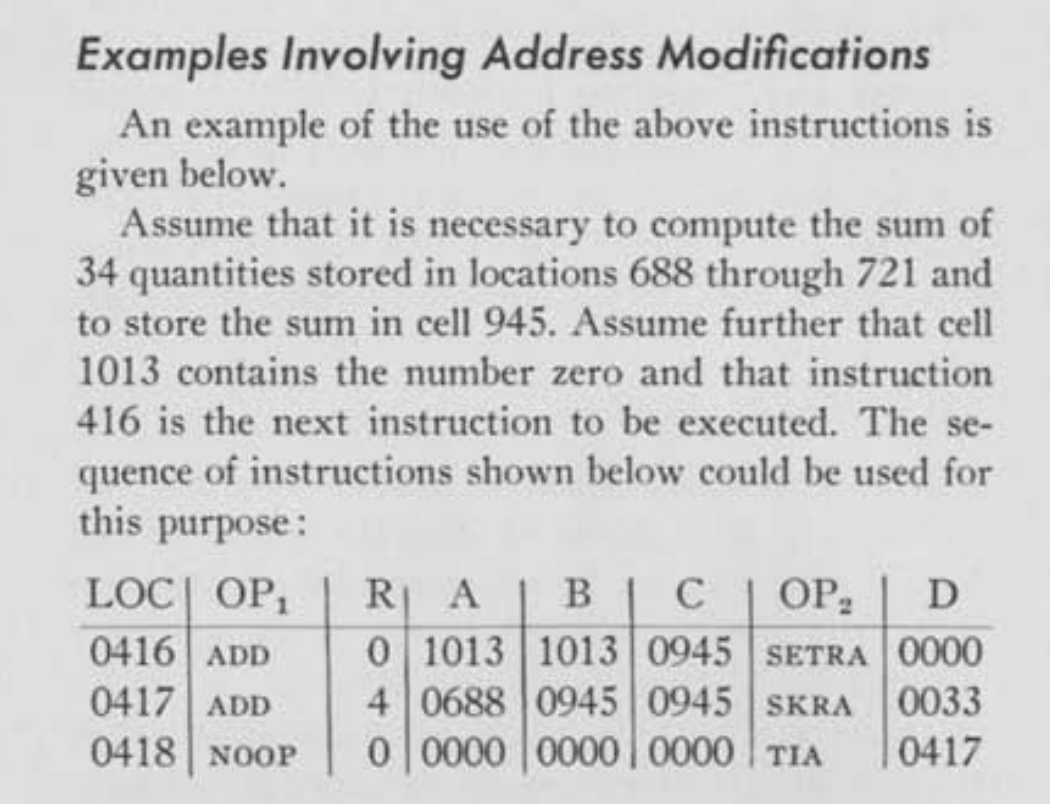
\includegraphics[width=0.5\linewidth]{resource/ibm-speedcoding-example.png}
  \caption{Excerpt from \textit{IBM Speedcoding for the Type 701
    Electronic Data Processing Machine}
  \cite{IBM_1954_Speedcoding}}
  \label{fig:ibm-speedcoding-example}
\end{figure}

Backus did not think all that highly of Speedcoding in retrospect, though it
gained traction in large part due to IBM's marketing power and the number of
users of the 701 relative to the size of the computer market at the time
\cite{Backus_1980_Programming_in_America_in_1950s}. It is unclear whether
Backus's assessment of his own code is accurate or if it's born of humility.

\begin{quotation}
  The success of some programming systems depended on the number of machines
  they would run on. Thus, an elegant system for a one-of-a-kind machine might
  remain obscure while a less-than-elegant one for a production
  computer achieved
  popularity. This point is illustrated by two papers at the 1954 ONR symposium
  One, by David E. Muller, describes a floating point interpretive system for
  the ILLIAC designed by D. J. Wheeler. The other, by Harlan Herrick and myself,
  describes a similar kind of system for the IBM 701 called Speedcoding. Even
  today Wheeler's 1954 design looks spare, elegant, and powerful, whereas the
  design of Speedcoding now appears to be a curious jumble of compromises.
  Nevertheless, Wheeler's elegant system remained relatively obscure (since only
  ILLIAC users could use it) while Speedcoding provided enough conveniences,
  however clumsily, to achieve rather widespread use in many of the eighteen 701
  installations.
\end{quotation}

In 1953, based on his experience with Speedcoding on the 701, Backus proposed
yet another language to elevate the programming experience on the 704. IBM
management supported the proposal. He formed a ten-person team of his own
choosing based out of IBM's Manhattan headquarters, including Irving Ziller,
\todo{list other members}. They released \textit{Preliminary Report,
  Specifications for the IBM Mathematical FORmula TRANslating System,
FORTRAN}\cite{IBM_1954_FORTRAN_Specifications} after about one year of working
together. Roughly two years after its first conception, \FTN{} was released for
the first time. It would go on to ship with every IBM 704 and become the
primary means of programming in the scientific community. Backus could not
stand how slow programming was without a higher-level language, and machines
were expensive; leasing a machine and spending time programming in machine code
wasted money compared to a compiler capable of generating reasonable machine
code (though at the time it usually underperformed hand-written code). Backus
and his team would continue to develop and stabilize this compiler for several
years, though.

\begin{quotation}
  \FTN{} did not really grow out of some brainstorm about the beauty of
  programming in mathematical notation; instead it began with the recognition
  of a basic problem of economics: programming and debugging costs already
  exceeded the cost of running a program, and as computers became faster
  and cheaper this imbalance would become more and more intolerable. This
  prosaic economic insight, plus experience with the drudgery of coding, plus
  an unusually lazy nature led to my continuing interest in making
  programming easier.
  This interest led directly to work on Speedcoding for the 701
  and to efforts to have floating point as well as indexing built into the 704.
  \cite{Backus_1980_Programming_in_America_in_1950s}
\end{quotation}

When Backus was forming his team in January of 1954, he was moved from the Pure
Science department at IBM into the Applied Science department because his boss
Rex Seeber wanted nothing to do with the project. There he found Irving Ziller,
who became his first teammate. By April, they had been joined by Harlan Herrick
who co-authored the Speedcoding paper with Backus at the ONR symposium
\citetitle{Backus_Herrick_1954_Speedcoding} in which they observe:

\begin{quotation}
  The question is, can a machine translate a sufficiently rich mathematical
  language into a sufficiently economical program at a sufficiently low cost to
  make the whole affair feasible?  consider the advantages of being
  able to state
  the calculations\dots for a problem solution in a concise, fairly natural
  mathematical language.
\end{quotation}

The reader should note that it is often incorrectly asserted (at times even by
Backus himself\cite{Backus_1980_Programming_in_America_in_1950s}) that this
came \textit{after} Backus and Ziller had been given a demonstration of Laning
and Zierler's algebraic compiler for the Whirlwind at MIT at the ONR symposium
of 1954. When they received this demonstration, there were already four members
of the \FTN{} team, Irving Ziller, Robert Nelson, Harlan Herrick, and Backus
himself. In Backus's words\cite{Backus_1980_Programming_in_America_in_1950s}:

\begin{quotation}
  The article and the letter therefore show that, much to my surprise, the
  FORTRAN effort was well under way before the ONR symposium and that,
  independently of Laning (but later), we had already formulated more ambitious
  plans for algebraic notation (e.g., Gail bjk) than we were later to find in
  Laning and Zierler's report and see demonstrated at MIT. It is therefore
  unclear what we learned from seeing their pioneering work, despite my mistaken
  assumption over the years that we had gotten our basic ideas from them
\end{quotation}

Indeed, even Grace Hopper at a 1956 symposium made the same assertion:

\begin{quotation}
  A description of Laming and Zierler' s system of algebraic pseudocoding for
  the Whirlwind computer led to the development of Boeing 's BACAIC for the 701,
  FORTRAN for the 704, AT-3 for the Univac, and the Purdue System for the Datotron and. indicated the need for far more effort in the area of algebraic
  translators.
  \cite{Knuth_TrabbPardo_1976_Early_Development}
\end{quotation}

I am not sure who to believe either!

With the support of his new boss Cuthbert Hurd, his family, friends, and his
team, the first report of \FTN{} was released externally to 704 users. This
brought interest from a variety of users, many of whom offered up members of
their teams to help.

\section{\FTN{} Optimization and the First Users}

Setting aside the members of the "priesthood" of computing who were hostile to
the idea of compilers and making programming more accessible, the external
report on \FTN{} brought these contributors into the fold:
\begin{itemize}
  \item Walter Ramshaw at United Aircraft allowed Roy Nutt to work
    with the team; he
    eventually designed and implemented parts of the runtime and I/O features.
  \item Charles W. Adams allowed Sheldon Best to join the team on
    leave from MIT.
  \item Sidney Fernback at the Livermore Radiation Laboratory loaned
    out Bob Hughes.
  \item Harry Cantrell at G.E. was enthusiastic about the project.
\end{itemize}

The team was composed of the following 9 members: David Sayre, Harlan Herrick,
John Backus, Lois Haibt, Robert Nelson, Roy Nutt, Sheldon Best, Richard
Goldberg, and Peter Sheridan.

Most of the skepticism about \FTN{} came from the "priesthood," Backus's
facetious term for the "elite" programmers who thought programming needn't be
made accessible and compilers would never achieve the performance their of
hand-written code. This made the optimization of \FTN{} programs a high
priority for the team; to achieve the widest possible adoption, they would need
to convince even the skeptics that \FTN{} programs could be efficient. In
Backus's 1976 retrospective on programming in the
1950s\cite{Backus_1980_Programming_in_America_in_1950s}, he highlights the
optimization efforts of three members of the original team:

\begin{itemize}
  \item Nelson and Ziller optimized array indexing expressions and
    loop analyses.
    Backus specifies that they could "could move computations from the object
    program to the compiler" which appears to be the first instance of
    constant-folding in a compiler.
  \item Best optimized the use of index registers based on the
    expected hotness of the
    execution path. "As of 1970 there were no known provably optimal
    algorithms for
    the problem he dealt with; his methods were the basis of many subsequent
    storage-allocation algorithms and produced code that is very difficult to
    improve. (For more details of Best's methods see [4, pp. 510-5151.)"
\end{itemize}

This is, as far as I can tell, the first concerted effort to produce an
optimizing compiler.

\section{Language Specification and Backus-Naur Form}

\todo{explain BNF and lang specs, tie in with GH algol
work}\cite{Backus_1980_Programming_in_America_in_1950s}:
\begin{quotation}
The notation for syntax description known as BNF offers another example of a
development which began with a prosaic recognition of a need.
After involvement
with two language design efforts-FORTRAN and IAL (ALGOL 58)-it
became clear, as
I was trying to describe IAL in 1959, that difficulties were
occurring due to
the absence of precise language definitions. In a recent course on
computability given by Martin Davis, I had been exposed to the work of the
logician Emil Post and his notion of a "production." As soon as the need for
precise description was noted, it became obvious that Post's
productions were
well suited for that purpose. I hastily adapted them for use in
describing the
syntax of IAL. The resulting paper [5] was received with a
silence that made it
seem that precise syntax description was an idea whose time had
not yet come.
As far as I know that paper had only one reader, Peter Naur. Fortunately, he
had independently recognized the need for precision; he improved
the notation
(replacing oi: by I and := by : =), improved its readability by not
abbreviating the names of metavariables, and then used it to describe the
syntax of ALGOL 60 in the definitive paper on that language. He
thus proved the
usefulness of the idea in a widely read paper I and it was accepted.
\end{quotation}
% \begin{figure}[h!]
%     \centering
%     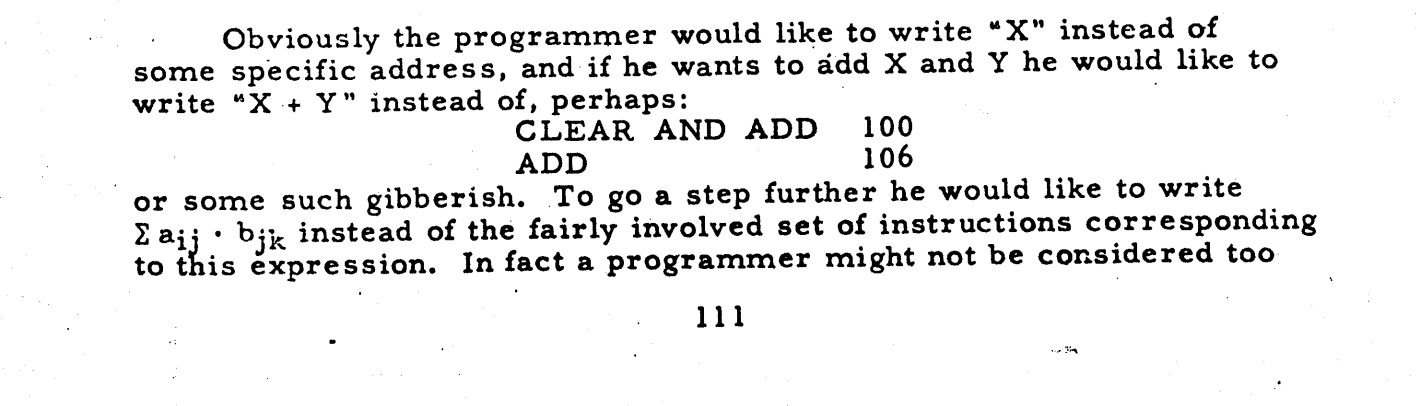
\includegraphics[width=0.5\linewidth]{resource/Backus_Herrick_Speedcoding_ONR_1954.png}
%     \caption{Excerpt from \citetitle{Backus_Herrick_1954_Speedcoding}}
%     \label{fig:backus-herrick-speedcoding-onr-1954}
% \end{figure}

\todo{Backus wasn't really that involved in fortran II and III and IV.
The rest of the team took over. He never wrote much fortran and
doesn't have many thoughts
about it today other that the "we should be making things higher level."}
\todo{Backus moved into functional programming. Was never fruitful.
He became a lab fellow at IBM after Watson Jr started the
fellowship program,
so he could kinda play with functional programming and not really
get much done.}
\todo{He didn't like Hopper's ideas for COBOL, thought they were
crazy and too complex.
Didn't like algol either. Really just wanted to make things
simpler and higher level
and easier to use. Pushed back against the priesthood.}
\todo{the priesthood didn't like fortran because it made things easy.
Backus resisted this urge at every point in his career.
Like GH, he wanted programming to be easy and accessible
(tho he didn't like her direction)}

\begin{quotation}
Though the FORTRAN operator's manual was completed by the fall of 1956, the
compiler itself was not distributed to IBM 704 installations
until April 1957.
Within a year after distribution, half of the IBM 704
installations were using
FORTRAN to solve more than half of all mathematical prob-lems.16
Subsequently,
compilers were produced for the IBM 705 and the IBM 650, quickly
making FORTRAN
the most widely used automatic program of its day. By 1961, UNIVAC users
demanded a compatible FORTRAN compiler and abandoned Hopper's MATH-MATIC.
\cite{grace_hopper_and_the_invention_of_the_information_age_2009}
\end{quotation}

\begin{quotation}
It describes the system which will be made available during late
1956, and is
intended to permit planning and fortran coding in advance of that
time [p. 1],
Object programs produced by fortran will be nearly as efficient as those
written by good programmers [p. 2], "Late 1956" was, of course, a
euphemism for
April 1957. Here is how Saul Rosen described fortran's debut [RO
64, p. 4]: Like
most of the early hardware and software systems, fortran was late
in delivery,
and didn't really work when it was delivered.
\cite{history_of_computing_in_the_twentieth_century_1980}
\end{quotation}

\begin{quotation}
It is not my intention to give a complete description of either; hence this
section will describe only the main highlights of FORTRAN development. The
earliest significant document that seems to exist 1s one marked
"PRELIMINARY REPORT, Specifications for the IBM Mathematical FORmula
TRANslating System, FORTRAN", dated November 10, 1954 and issued by the
Programming Research Group, Applied Science Division, of IBM.
\cite{sammet_programming_languages_history_and_fundamentals_1969}
\end{quotation}

\begin{quotation}
Laning and Zierler's algebraic compiler served as evidence that prestigious
institutions such as MIT were taking automatic programming
seriously, prompting
Backus to write Laning a letter shortly after the May symposium.
In the letter,
Backus informed Laning that his team at IBM was working on a
similar compiler,
but that they had not yet done any programming or even any
detailed planning.12
To help formulate the specifications for their proposed language, Backus
requested a demonstration of the algebraic compiler, which he and Ziller
received in the summer of 1954. Much to their dismay, the two
experienced firsthand the efficiency dilemma of compiler-based
language design. The MIT
source code was commendable, but the compiler slowed down the Whirlwind
computer by a factor of 10. Since computer time was so dear a
commodity, Backus
realized that only a compiler that maximized efficiency could
hope to compete
with human programmers. Despite this initial disappointment, Laning and
Zierler's work inspired Backus to attempt to build a compiler that could
translate a rich mathematical language into a sufficiently
economical program
at a relatively low cost.13
\cite{grace_hopper_and_the_invention_of_the_information_age_2009}
\end{quotation}

\section{The IAL and the ALGOrithmic Language}

Before Hopper, Mayes and Phillips pulled together their committees for a common
business language, design-by-committee was already in the academic milieu,
especially in Europe.
While not commercially successful, ALGOL introduced a number of important concepts
like block scopes and the declaration of the types of variables, and it would
go on to be the standard language for describing algorithms in academia.
Originally called IAL (International Algebraic Language), it came to be called
ALGOL, or ALGOrithmic Language, and was designed by an international committee
with representatives from different organizations with the goal of a truly
machine-independent language.

After deliberation in numerous committees, representatives from the German
Association for Applied Mathematics and Machinery (GAMM) and the ACM met in
Zurich, Switzerland in the summer of 1958. They had both produced similar
reports and wanted to meet and agree on a unified language.
John Backus, Charles Katz, Alan Perlis and Joseph Wegstein from the ACM attended this meeting.
\todo{who were these people? Add some narrative. Maybe of Naur, then tie in with Backus.}
They arrived at the following objectives
\cite{perlis_samelson_1958_preliminary_report_ial}:

\begin{enumerate}
\item The new language should be as close as possible to standard mathematical 
      notation and be readable with little further explanation.
\item It should be possible to use it for the description of computing processes in publications.
\item The new language should be mechanically translatable into machine programs.
\end{enumerate}

Shortly thereafter, a large number of dialects and partial implementations sprung up around Europe
and the US such as BALGOL from Burroughs Corporation in Detroit, Michigan for the Burroughs 220.
Manufacturers such as Burroughs found the standard to be insufficient for their users:
"BAC-220 provides additions for the ALGOL reference language which are essential to
the operation of data-processing systems: input-output
facilities, conventions for inclusion of segments of machine-language coding,
and diagnostic features" \cite{burroughs1963bac220}.
This was intentional; the specifications of ALGOL (both the 1958 and the 1960 versions)
was solely for the purposes of
describing computation; no I/O or system libraries were specified.
Other dialects included CLIP, JOVIAL, MAD, and NELIAC.
The first issue of the \textit{ALGOL Bulletin} was issued in March of 1959 out of Copenhagen
with Peter Naur as the editor.

Jean Sammet describes the impact of ALGOL 58
\cite{sammet_programming_languages_history_and_fundamentals_1969}:
\begin{quotation}
Among the more intriguing technical features of ALGOL 58 were its essential 
simplicity; the introduction of the concept of three levels of language, namely 
a reference language, a publication language, and hardware representations; the 
\textbfit{begin\dots end} delimiters for creating a single (compound) statement from simpler 
ones; the flexibility of the procedure declaration and the \textbfit{do} statement for 
copying procedures with data name replacement allowed; and the provision for 
empty parameter positions in procedure declarations. While ALGOL 58 is not an 
exact subset of ALGOL 60, the only items of significance which are in the 
former but not the latter are the \textbfit{do} which was removed as a concept (although 
the word was used for something else) and the empty parameter positions. 
Because of this major carry-over, specific technical description of ALGOL 58 is 
not necessary. 
\end{quotation}

\section{ALGOL 60}

\todo{backstory of Peter Naur}

The International Conference on Information Processing was held in Paris
in June, 1959, where there were several key developments in ALGOL.
Firstly, John Backus presented the now-famous paper on Backus-Naur Form
for formal specification of programming languages\cite{backus_ial_1959}.
Although other accounts describe this paper as having garnered significant
attention in the IAL proceedings, Backus would recount that his paper
"was received with a silence that made it seem that precise syntax
description was an idea whose time had not yet come.
As far as I know that paper had only one reader, Peter Naur"
\cite{Backus_1980_Programming_in_America_in_1950s}.
Backus was involved in two programming languages at the time, \FTN{} and IAL,
having already moved on from Speedcoding.
Backus had been made aware of the logician Emil Post and her work on computability
in a course given by Martin Davis, in particular, Post's notion of a "production."
It was this concept that inspired Backus to write the 1959 paper, and Naur
would go on to extend it. This is part of Backus's specification of arithmetic expressions
in the paper before Naur's changes\cite{backus_ial_1959}:

\[
\langle \textit{factor} \rangle :\equiv
\langle \textit{number} \rangle \;\overline{\text{or}}\;
\langle \textit{function} \rangle \;\overline{\text{or}}\;
\langle \textit{variable} \rangle \;\overline{\text{or}}\;
\dots
\]

Naur would make the notation more readable by replacing $\overbar{or}$ with $|$
and $:\equiv$ with $::=$ and by fully spelling out names that backus had abbreviated.
Naur's edits and extensions would bring interest from more readers than Backus's original paper had.
This form would come to be known as Backus-Naur Form, or BNF.
Naur would submit this in a paper to the subsequent ALGOL meeting in 1960,
titled \citetitle{naur_backus_algol_1960}\cite{naur_backus_algol_1960}.
Various commitees had established some shortfalls of the original design of the AIL,
and the 1960 meeting set out to address them with the help of Backus and Naur's
specification.
This report "represents the union of the Committee's concepts and the
intersection of its agreements."
The IAL had been renamed ALGOL 58 and then finally ALGOL 60 in Naur's report.

The final report specified expressions to have the following syntax:

\[
\langle \textit{expression} \rangle ::=
\langle \textit{arithmetic expression} \rangle
| \langle \textit{Boolean expression} \rangle
| \langle \textit{designational expression} \rangle
\]

\section{Adoption of ALGOL}

The \textit{ACM Communications} started publishing an \textit{Algorithms} section;
ALGOL 58 was initially used, but ALGOL 60 was adopted once the updated report
was in wide circulation.
\FTN was not considered acceptable for publication until 1966, and even then
it did not see widespread use in the journal.
Because ALGOL had been designed from scratch by committee, there were
no reference compilers for people to use; the only way to verify the correctness
of an algorithm described in ALGOL was to rewrite it in another language
and run test against test cases.

In early 1960, the \textit{ACM ALGOL Maintenance Group} formed: an informal working
group for the purpose of discussing the implementation of an ALGOL compiler.
They discussed ambiguities in the specification and potential changes to the ALGOL 60 report.
They mostly corresponded by mail and reports of their discussions were synthesized in
the \textit{ALGOL Bulletin}\cite{sammet_programming_languages_history_and_fundamentals_1969}.
The 14 issue of the bulletin in 1962 contained a questionnaire from Peter Naur
about some ambiguities in the 1960 report, and the philosophy of some proposed changes and
enhancements to the language.
\footnote{The reader may find it interesting that in this edition of the bulletin,
Jean Sammet submitted a paper on \textit{A Method of Combining ALGOL and COBOL};
\todo{follow up on this?}}
This questionnaire was used as a guide for another committee meeting in Rome in April of 1962
the primary result of this meeting is detailed in Naur's
\citetitle{naur_revised_report_algol_1962}.

\section{Peculiarities of ALGOL}

The reader may find it interesting that ALGOL had a number of peculiar features.
Namely, the distinction between \textit{call by name} and \textit{call by value}.
Naur's 1962 revised report explains it best, I think\cite[Section 4.7.3]{naur_revised_report_algol_1962}:

\begin{quotation}
\noindent
\textbf{4.7.3.1 Value assignment (call by value)}

of the corresponding actual parameters\dots the effect is as though an 
additional block embracing the procedure body were created in which these 
assignments were made to variables local to this fictitious block\dots

\noindent
\textbf{4.7.3.2 Name replacement (call by name)}

Any formal parameter not quoted in the value list is replaced, throughout the 
procedure body, bu the corresponding actual parameter, after enclosing this 
latter in parentheses wherever syntactically possible.
\end{quotation}

While neither Naur's revised report nor Edgar Dijkstra's
\citetitle{dijkstra_primer_of_algol_programming_1962}
point out the implications of this distinction, it is important to note
the subtle implications.
Call-by-name is not common in modern programming languages, and readers
may find it more similar to macro expansion
(though it is not, in fact, simply textual replacement).
The following example illustrates the difference:

\lstinputlisting[language=python,frame=single]{chapters/dawn/callbyname1.py}

Most implementations of call-by-name use zero-argument thunks to delay
the evaluation of arguments until they are used in the body.
The arguments to function calls become zero-argument closure functions
returning the value of the argument expression and capable of being
\textit{l-values}, or values in the left-hand side of an assignment expression.
Then, each instance of the argument in the callee's body is replaced
with an invocation of this function such that it is evaluated anew
each time it appears.
The prior Python example may be rewritten to emulate call-by-name as follows:

\lstinputlisting[language=python,frame=single]{chapters/dawn/callbyname2.py}

Call-by-value semantics demand that the argument to \texttt{double} be evaluated
before entering the function, so \texttt{get\_5} is called once and
\textit{the result} is passed to \texttt{double}.
With call-by-name semantics, \texttt{get\_5} is passed the expression itself,
which is the substituted into the body of the callee \textit{before}
being evaluated.

Donald Knuth proposed the \textit{man or boy} test in the \textit{ALGOL Bulletin}
to distinguish between
conformant ALGOL compilers capable of handling recursion and non-local references
using call-by-name semantics\cite{Knuth1964ManOrBoy}.

\begin{quotation}
There are quite a few ALGOL60 translators in existence which have been designed 
to handle recursion and non-local references properly, and I thought perhaps a 
little test-program may be of value. Hence I have written the following simple 
routine, which may separate the man-compilers from the boy-compilers.

This uses nothing known to be tricky or ambiguous. My question is: What should 
the answer be? Unfortunately, I don't have access to a "man-compiler" myself, 
asn do I was forced to try hand calculations. My conjecture (probably wrong) is 
that the answer will be

\[
73 - 119 - 177 + 102 = -121 .
\]

I'd be very glad to know the right answer.
\end{quotation}

The program is as follows:

\lstinputlisting[language=algol,frame=single]{chapters/dawn/knuth-man-boy-test.a68}

There are some useful applications of call-by-name semantics as well;
it is not \textit{solely} an avenue for confusion.
Jensen's Device, named in honor of Mr. J. Jensen of Regnecentralen, Copenhagen,
is a well-known application of call-by-name semantics.
This allows the user of a function to describe an expression to be evaluated
in a loop body inside the function, permitting a very general summation function.
There is not an especially elegant way to do this in a call-by-value language,
but as Dijkstra points out\cite{dijkstra_defense_of_algol_60_1961},
it can be implemented with this ALGOL program:

\lstinputlisting[language=algol,frame=single]{chapters/dawn/jensens-device.a68}

To simply sum the values of the array \texttt{V} from 1 to 100, one would call:
\texttt{Sum(i, 1, 100, V[i])}.
The real power of this device is its generality;
if a user were to need to compute $\sum_{i=1}^{100} V_{i}\times i$,
they could call \texttt{Sum(i, 1, 100, V[i]*i)}.
The first and final arguments to this function are not evaluated
until they are used in the body of the loop in \texttt{Sum}.
Others have also pointed out numerous easy-to-make mistakes
that arise because of this feature.
For example, a naive implementation of a swap function may easily
cause unintended side effects:

\lstinputlisting[language=algol,frame=single]{chapters/dawn/swap-error.a68}

While calling \texttt{Swap(i, j)} may work correctly, calling
\texttt{Swap(i+1, j+1)} or \texttt{Swap(A[i], A[j])} would not.

Among the now-unusual argument evaluation semantics, ALGOL also lacked any I/O 
facilities as we have already discussed.  The language also made string 
variables available, but provided no means of manipulating them.  ALGOL 
permitted \textit{own variables}, which are akin to static variables in C or 
SAVE variables in \FTN{}; they retain their values between entrances to the 
block.  Dijkstra also points out nowhere is the evaluation order of 
subexpressions specified\cite{dijkstra_defense_of_algol_60_1961}.

While the declared intent of defining a language detached from any particular
manufacturer or machine was laudable (and profitable in the case of portable 
languages to follow), ALGOL was so far removed from the machine to be useless without
supplementary libraries (for I/O, string processing, etc).

\section{ALGOL R, S, W, X, Y, and W}

For years after the 1962 Rome meeting, there were discussions amongst the ALGOL
community about potential changes and improvements to the language.
The 1960 and 1962 meetings restricted themselves to clarifying ambiguities
and rectifying true errors in the prior reports, but not extensions or
significant changes.
In the spring of 1968, a draft report of such an extension to the language 
was released with Adriaan van Wijngaarden as the editor.
The first programming language designed by international committee received
significant interest and is still used in academia today, however it never
gained significant traction.
Outside of small snippets in academic papers, it was only ever in use by
the Burroughs Corporation\cite{burroughs1963bac220},
and their implementation required significant library
development to provide their programers with an environment capable of doing
much of anything useful.

The computer and aerospace historian Paul Ceruzzi describes the result of
the ALGOL 68 report as follows:

\begin{quotation}
Whereas ALGOL-60 was based on a formal structure
and was very lean, ALGOL-68 was burdened by an attempt to do too
much, with the effects that some features interfered with the clean
implementation of others. It was hard to understand. In an attempt to
satisfy a broad range of users worldwide, the committee produced
something that satisfied few.
\end{quotation}

\todo{Honestly the wikipedia is really good for this one.
March 1964, follow up to Rome meeting. They agreed to start on ALGOL X and ALGOL Y.
Read \citetitle{a_history_of_algol_68_1993}.}
\todo{Defined in Wijngaarden Grammar by Adriaan van Wijngaarden.
Contains parsing and things which in other langauges are called semantics.}

\todo{'68 critcized by Hoare and Dijkstra for abandoning simplicity of '60.
In 1970, ALGOL 68-R became the first working compiler for ALGOL 68.
ALGOL 68 also had a notable influence in the Soviet Union, details of which can be found in Andrey Terekhov's 2014 paper: "ALGOL 68 and Its Impact on the USSR and Russian Programming."}

\section{ALGOL 68 and ALGOL's Legacy}

\todo{Pascal, Ada}

\begin{quotation}
An interesting observation is the fact that the two-level formalism used
in the description of ALGOL 68 by itself led to a number of programming
languages, including PROLOG (Colmerauer) and my own CDL family (Compiler
Description Language).
\citetitle{a_shorter_history_of_algol68_1994}
\end{quotation}

\pagebreak
\section{Timeline}
\pagebreak
\begin{figure}[h]
\begin{luacode}
timeline.draw_timeline({ 
    start_year = 1942,
    end_year = 1957,
    marker_interval = 1,
    show_year = false,
    events = {
        {1942, "Zuse conceptualizes first high-level language \\textit{Plankalkül}"},
        {1944, "Automatic Sequence Control Calculator started working"},
        {1950, "Rutishauser ran the Z4 as a compiler at ETH", position=1950},
        {1951, "B{\"o}hm develops practical compiler for PhD thesis at ETH"},
        {1951.5, "Hopper begins work on the A-0 compiler for the UNIVAC I"},
        {1952, "Hopper presents \\textit{Automatic Programming} at ACM"},
        -- {1952.5, "Alick Glennie develops first compiler in the modern sense for the U of Manchester Mark I"},
        {1952.5, "Alick Glennie develops compiler for Mark I "},
        {1953, "Hopper's team completes the A-1"},
        {1953.3, "Hopper's team completes the A-2"},
        {1953.6, "Hopper gives presentation to UNIVAC users on the A-2"},
        {1953.9, "Numerous US government agencies have adopted the A-2"},
        {1954.5, "John Backous at IBM begins work on \\ftn{}"},
        {1954.9, "Nora Moser of US Army sends Hopper modifications to the A-2"},
        {1957, "John Backous at IBM released the first \\ftn{} compiler, the first commerical compiler"},
    },
})
\end{luacode}
\caption{Early compiler history, 1940--1960}
\label{fig:dawn-timeline}
\end{figure}

